\section{Advanced Models}
%With the question defined, the equations of motion derived, we can now consider the different models to achieve maximum displacement from a single jump.
%
%% TODO: maybe put the constants before engine section
%\subsection{Constants}
%One might notice that I've deliberately left some of the constants $j_i$ clear of meaningful values and only suggested in-game default values. This is because many long-jumpers in the community find the default (vanilla) settings of the game engines ``bland'', reducing the excitement of this activity. Therefore, I will be setting some of the engine constants myself.
%
%There are 4 of them:
%\begin{itemize}
%    \item \verb|sv_gravity| ($g$), set to 800
%    \item \verb|sv_maxspeed| ($L$), set to 250
%    \item \verb|sv_airaccelerate| ($A$), set to 10
%    \item \verb|tickrate| ($n$), set to 64, or $\tau=\frac{1}{64}$
%\end{itemize}
%
%The only meaning deviation from the default settings are the speed limit $L$, for the default settings limits the optimization one can achieve, while the higher value of $250$ simply magnifies the result that one can achieve.
%
%Furthermore, all models are free to set the initial velocity $\tv_0$, with the constraint that the magnitude of $\tv_0$ does not exceed $250$, the speed limit.
%
%% TODO: maybe change this to Euler-Lagrange? Because it uses the diff equations
%\subsection{Straight line}
%% where you do nothing
%We all know the fastest route (shortest distance) from point $A$ to point $B$ is with a straight line connecting $A$ to $B$. Therefore if the velocity magnitude is maximized, and as time is proportional to distance: $t = \frac{s}{\tmag{\tv}}$, it seems that a straight line would maximize the jumping distance assuming no constraints. This will serve as a good baseline for all the other models.
%
%I have decided for the player to travel along the y-axis because I personally find it nicer to graph and draw with, but all maths would apply if you wish to substitute for the x-axis. This is represented by the acceleration function:
%
%\begin{figure}[H]
%    \centering
%    \[
%    \tunit{a}(t) = \tang{0, 1}
%    \]
%    \caption{The straight line model}
%\end{figure}
%
%Notice that player acceleration is constant in this model, and which can be achieved simply by looking forward, and press the key $w$ during the jump. Furthermore, we can set the initial velocity to point directly upwards in the y direction, such that:
%\[
%\tv_0 = \tang{0, 250},
%\]
%for common knowledge tells me that a faster initial speed in the direction where I am going will result in higher overall travel distance. Overall, there exists four metrics for each model, each worth evaluating.
%
%We can first look at the case without the max speed constraint. By running a simulation with the engine constants discussed before, I got a result of $\approx 807.5$ hammer units in a jump. Predictably, this model will have the player traveling in a straight line (figure \ref{fig:straight_nothing_1}).
%
%\begin{wrapfigure}{r}{0.48\textwidth}
%    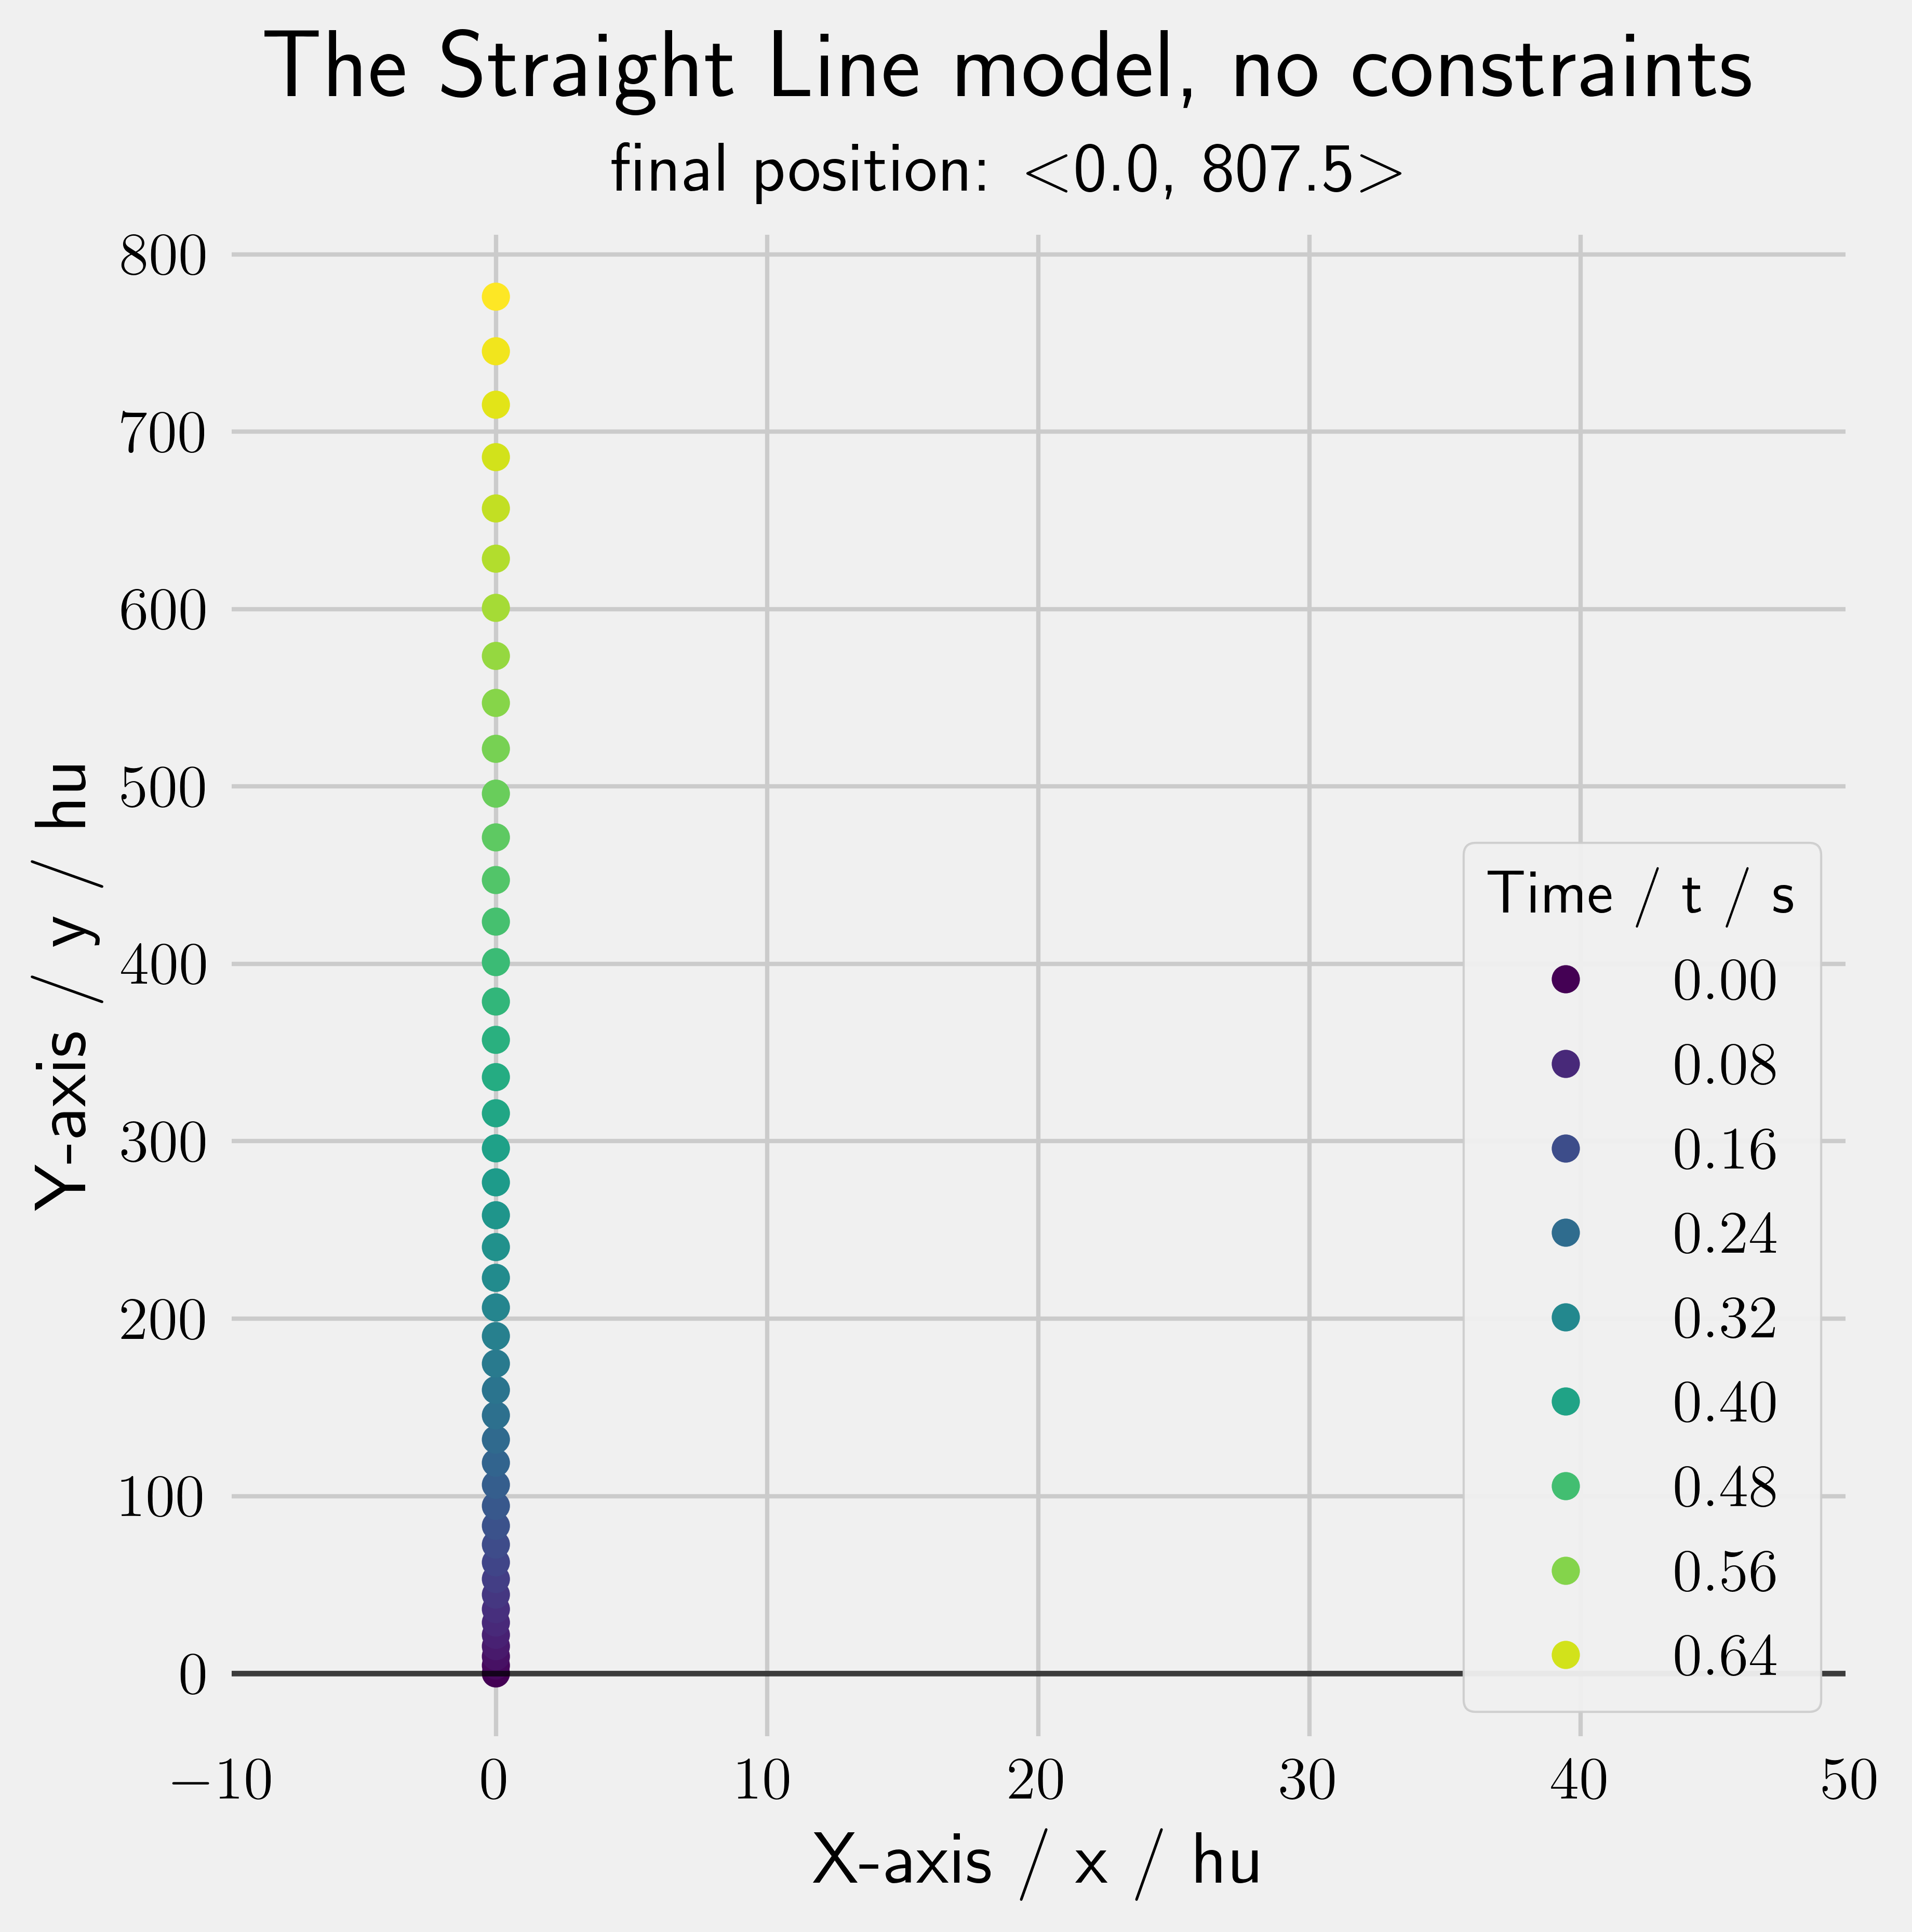
\includegraphics[width=0.45\textwidth,right]{assets/straight_nothing_1.png}
%    \caption{}
%    \label{fig:straight_nothing_1}
%\end{wrapfigure}
%
%I can comfortably say that this jumping distance would never be possible to achieve in game, for this model can be proven to be the most optimal jumping path if there are no speed limits (appendix, using EL equation). This number of around $800$ hammer units serves to be the upper-bound output of our optimization, and the lower-bound being its negative of around $-800$ (if you wish to accelerate directly backwards with negative initial velocity).
%
%Additionally we can also utilize the equation derived in the last section (equations \ref{eq:jumping}).
%
%Using the acceleration function, we can define $x(t)$ and $y(t)$ as:
%\[
%    x(t) = 0, \quad y(t) = 1.
%\]
%
%Their first and second order indefinite integrals can be obtained using calculus:
%\begin{alignat*}{3}
%    X(t) &= \int x(t) \, dx = 0, \quad
%    &&\tfx(t) &&= \int X(t) \, dx = 0\\
%    Y(t) &= \int y(t) \, dx = t, \quad
%    &&\tfy(t) &&= \int Y(t) \, dx = \frac{1}{2} t^2,
%\end{alignat*}
%notice that the constants during integration are omitted as we've incorporated them into the derivation of the jumping motion equations as $c_1$, and $c_2$.
%
%Therefore the $x$ position after $t_f$ seconds assuming no speed limit is:
%\begin{align*}
%    p_x &= p(t_f)_x = w\tfx(t_f) + t_f(v_{0x} - w\tfx'(0)) - w\tfx(0)\\
%    &= w \times 0 + t_f(0 - w \times 0) - w \times 0\\
%    &= 0,
%\end{align*}
%and the respective $y$ position is:
%\begin{align*}
%    p_y &= p(t_f)_y = w\tfy(t_f) + t_f(v_{0y} - w\tfy'(0)) - w\tfy(0)\\
%    &= w \frac{1}{2} t_f^2 + t_f(v_{0y} - w v_{0y} \times 0) - w \times 0\\
%    &= (10 \times 250) \frac{1}{2} (0.7)^2 + 0.7 \times 250\\
%    &= 787.5
%\end{align*}
%
%% TODO: change A to 10
%
%The jumping motion differential equations resulted in a similar sized jumping distance in comparison to the engine simulated $\approx807.5$. I believe that a $\frac{|787.5-807.5|}{807.5} \approx 2.48\%$ error is a very well approximation of this continuous method for future modeling.
%
%\begin{wrapfigure}{r}{0.48\textwidth}
%    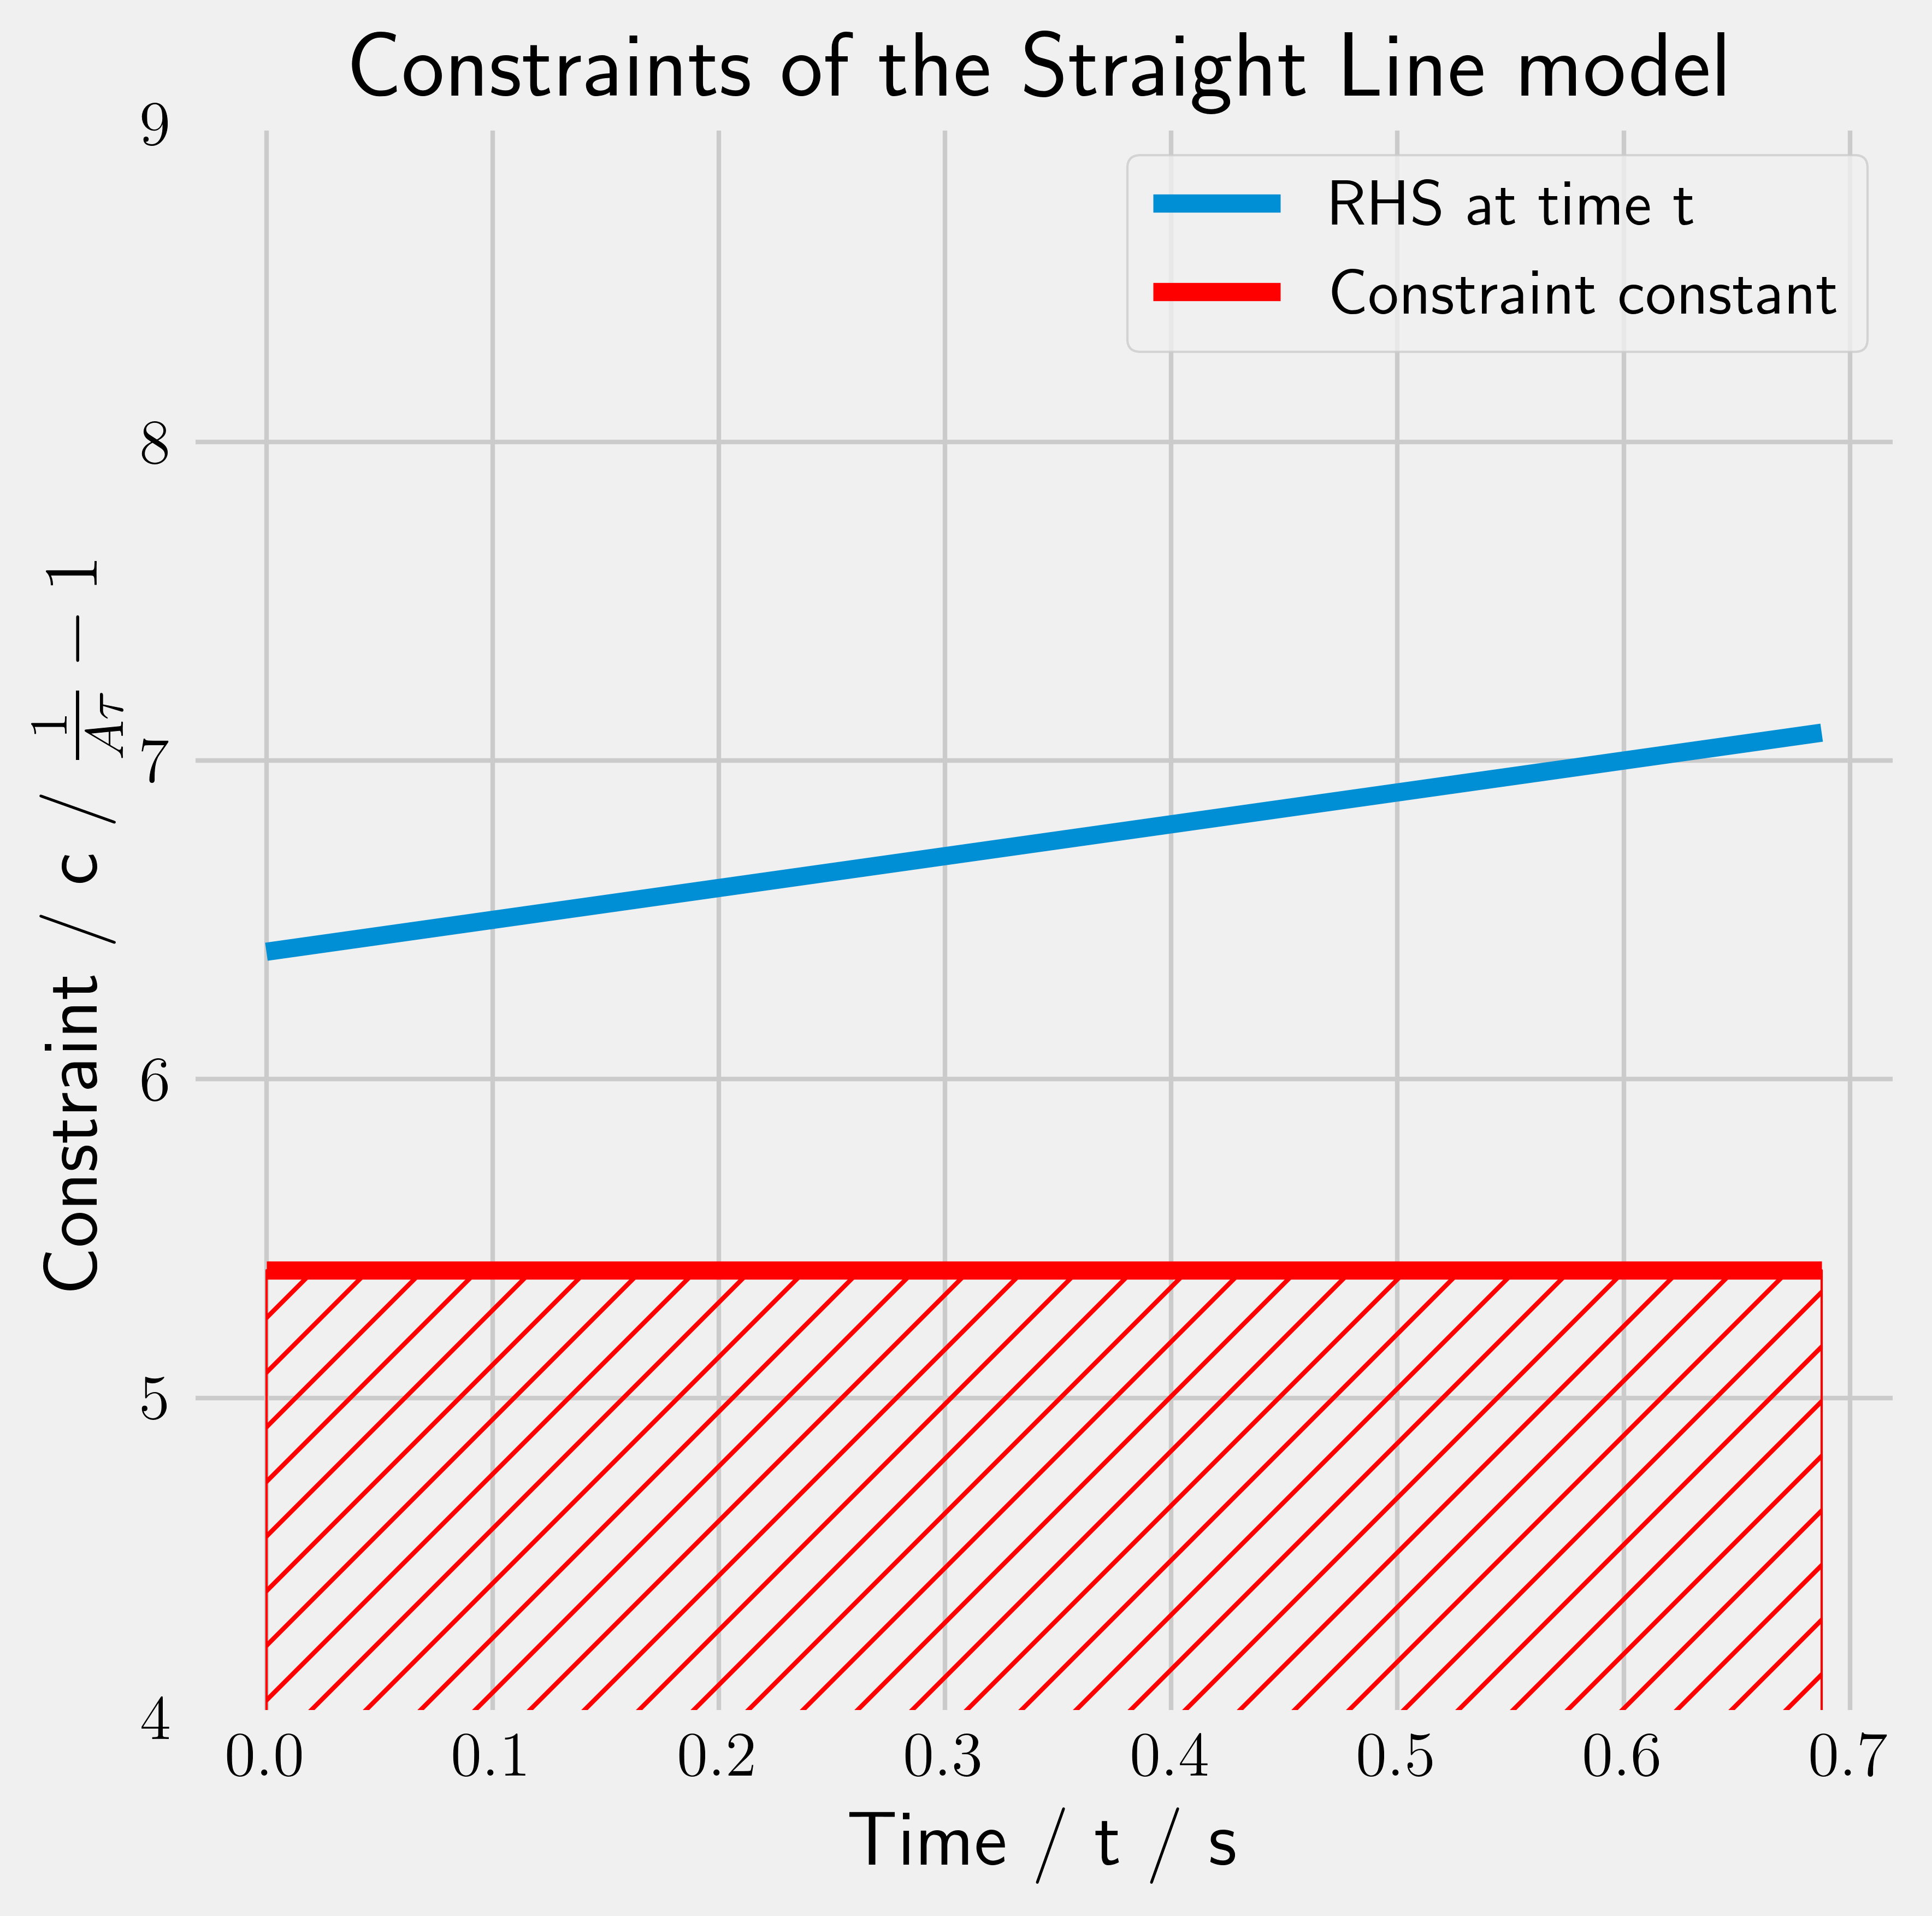
\includegraphics[width=0.45\textwidth,right]{assets/straight_constraint_inequality.png}
%    \caption{}
%    \label{fig:straight_constraint_inequality}
%\end{wrapfigure}
%
%But the game analyzed does have the constraint of a speed limit so players cannot accelerate infinitely, traveling across the map in two-to-three seconds. The graphing of the constraint (equation \ref{eq:constraint}) shows the problems (figure \ref{fig:straight_constraint_inequality}).
%
%It is obvious that the RHS (top line) is higher than the constraint LHS (bottom shaded area). This indicates that the player exceeds the speed limit for every time within the considered time domain, which will undoubtedly massively decrease the restricted displacement. The inequality of the RHS can be represented symbolically by substitution of the player acceleration function into equation \ref{eq:constraint}:
%\[
%    5.4 \ge t + \frac{v_{0y}}{w}.
%\]
%
%Because the variable $\frac{v_{0y}}{w} = 6.4$, the inequality will only hold in negative $t$, which is not in the time domain considered. Only when the initial y-axis velocity is below $\frac{5.4 w}{v_{0y}}$ would there be acceleration on the first frame.
%
%Therefore the restricted player motion would be without any acceleration at any time. The continuous displacement of the player at time $t_f$ can be computed by setting the variable $w=0$, or:
%\begin{align*}
% \tp(t)_x &= t v_{0x} = 0\\
% \tp(t)_y &= t v_{0y}\\
% \tp(t_f)_y &= 0.7 \times 250 = 175.
%\end{align*}
%
%The discrete restricted jumping equation using Euler's method (figure \ref{eq:rje}) resulted in a similar distance of $175.78$, using constant $h=\tau$. Furthermore I've noticed that the displacement/time graph (figure \ref{fig:straight_constraint}) have displacements equality spaced in the y-axis --- in contrast with the ever expanding dots in the unrestricted case (figure \ref{fig:straight_nothing_1}). I believe that this indicates a lack of acceleration, which greatly reduced the result of this baseline model. Furthermore, the lack of acceleration means that this model can also be achieved with no player inputs, as the minimum value of acceleration $w$ is zero.
%
%\begin{wrapfigure}{r}{0.48\textwidth}
%    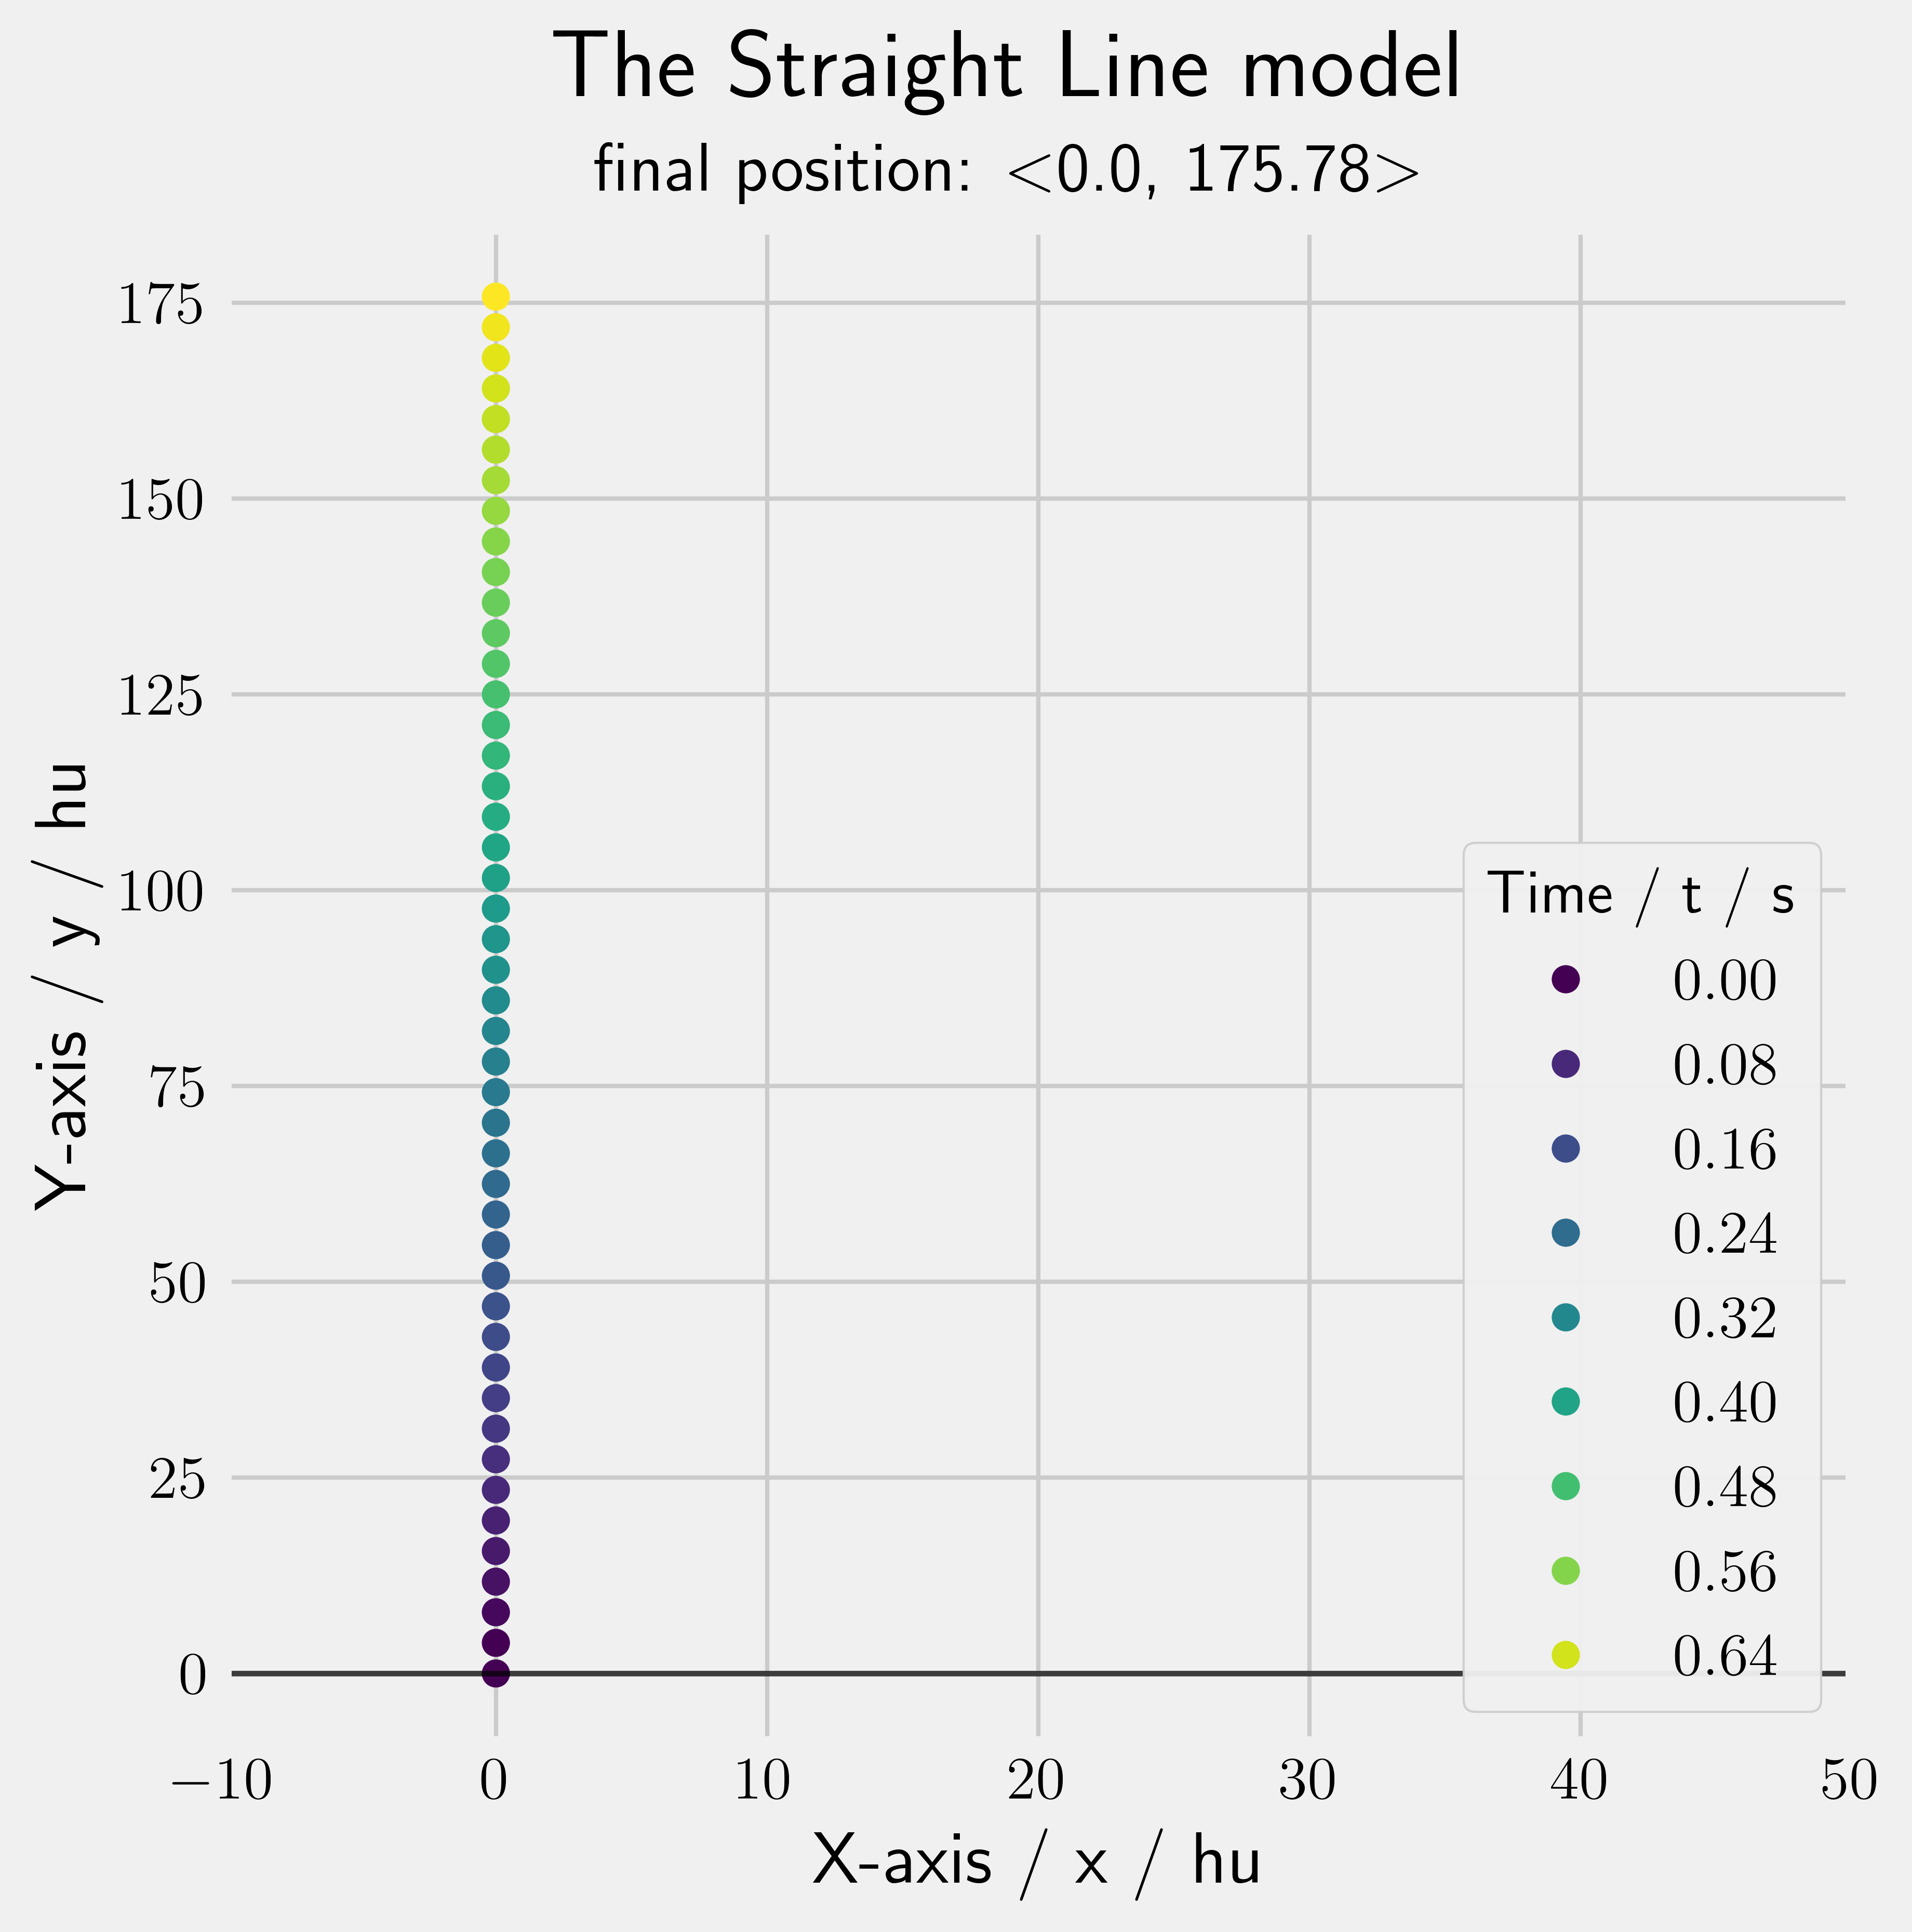
\includegraphics[width=0.45\textwidth,right]{assets/straight_constraint.png}
%    \caption{}
%    \label{fig:straight_constraint}
%\end{wrapfigure}
%
%Overall, the straight-line model establishes the baseline of my analysis. Using this strategy, the player has traveled an average distance in a jump of around $175$ hammerunits, which is well below what I can achieve in-game. The method has the benefit of requiring no input from the player, and can be performed consistently every  time. This makes the method the best model to conserve human energy by minimizing the amount of effort. But we can do better.

% conclusion

% Do not have enough words for this machine learning step
%\subsection{Machine learning}
%To kick start the optimization step, I decided to utilize the computing power I have access to to run a machine learning model on this problem. The result of which can potentially be graphed and fitted a model against, which could potentially be optimized further.

%From my previous experience in strafing sub-optimally, I hypothesize that

% state the steps of this

\subsection{Discrete model}
%My second model would be trying to optimize the y-axis displacement with each discrete change in time. Reflect back to subsection where I defined the restrictions (\ref{eq:constraint}), where the movement integrated vector functions must satisfy an inequality for maximum acceleration. This is problematic for this method in that the integrated player acceleration function $X(t)$ and $Y(t)$ have no obvious relationships, as it does not need to be a vector with unit length 1. I tried to define $x(t)$ in terms of $y(t)$ with
%\[
%    x(t) = \sqrt{1-y(t)^2},
%\]
%but found the integral
%\[
%    X(t) = \int \sqrt{1-y(t)^2} \, dt
%\]
%a pain or sometimes impossible to solve analytically. I needed to represent acceleration in another form preferably in a single variable function --- I attempted to do it with polar coordinates.
The key idea hypothesizes higher velocity with higher displacement, so does the same apply to acceleration as well? The discrete model considers the maximization of velocity by maximizing the acceleration at every frame.

However, a new framework in modeling the player's movement is needed. If we were to continue using the Cartesian axis for player direction $\td$, I could either model the two functions $\td_x(t)$ $\td_y(t)$ and ensure that they consulates a unit vector, which is complicated; or I can write an axis in terms of the other, like
\[
    \td_y(t) = \sqrt{1-\td_x(t)^2},
\]
but due to the velocity being the integral of acceleration and integrating such a function is difficult, it is also not ideal. So I came up with the idea of polar coordinates.


%I found the constraint equations to be difficult to use because it contains two related functions as input: $X(t)$ and $Y(t)$. This is because the solution to the problem is currently of form $x(t)$, which is the x component of acceleration as a function of time. Therefore the first integral $Y(t)$ must be in the form:
%\[
%    Y(t) = \int \sqrt{1-x(t)^2} \, dt,
%\]
%which turns out to be a very difficult integral to solve analytically. Therefore I attempted to derive the equations of motions again in polar coordinates, because I realized that I can represent player acceleration with a single function $\theta(t)$, which removes the square root function in the constraint inequality and allowing optimizations frame by frame.

% TODO: Finish writing this

\subsubsection{Polar equations of motion}
Let the player displacement $\tp(t)$, velocity $\tv(t)$ be complex numbers with the real part the x-axis and the imaginary part the y-axis. They are represented in Euler forms (where $\exp(x)= e^{x}$ for simplicity):
\begin{align*}
    \tp(t) &= a(t) \exp(b(t) \I)\\
    \tv(t) &= r(t) \exp(\phi(t) \I),
\end{align*}
where $a(t)$ and $r(t)$ are the magnitudes of the player displacement and velocity, and $b(t)$ and $\phi(t)$ are their respective angles from the x-axis.

\begin{figure}[H]
    \centering
    \sized[0.4]{
        \tikzset{every picture/.style={line width=0.75pt}} %set default line width to 0.75pt

        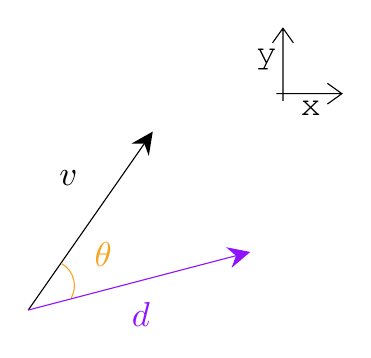
\begin{tikzpicture}[x=0.75pt,y=0.75pt,yscale=-1,xscale=1]
        %uncomment if require: \path (0,224); %set diagram left start at 0, and has height of 224

        %Shape: Axis 2D [id:dp14144095768588938]
        \draw [color={rgb, 255:red, 0; green, 0; blue, 0 }  ,draw opacity=1 ] (423.68,50.2) -- (455.25,50.2)(426.84,18.66) -- (426.84,53.7) (448.25,45.2) -- (455.25,50.2) -- (448.25,55.2) (421.84,25.66) -- (426.84,18.66) -- (431.84,25.66)  ;
        %Straight Lines [id:da47227000140678865]
        \draw    (304.12,154.45) -- (362.4,70.91) ;
        \draw [shift={(364.12,68.45)}, rotate = 124.9] [fill={rgb, 255:red, 0; green, 0; blue, 0 }  ][line width=0.08]  [draw opacity=0] (10.72,-5.15) -- (0,0) -- (10.72,5.15) -- (7.12,0) -- cycle    ;
        %Straight Lines [id:da6578973543629849]
        \draw [color={rgb, 255:red, 144; green, 19; blue, 254 }  ,draw opacity=1 ]   (304.12,154.45) -- (408.21,127.21) ;
        \draw [shift={(411.12,126.45)}, rotate = 165.34] [fill={rgb, 255:red, 144; green, 19; blue, 254 }  ,fill opacity=1 ][line width=0.08]  [draw opacity=0] (10.72,-5.15) -- (0,0) -- (10.72,5.15) -- (7.12,0) -- cycle    ;
        %Shape: Arc [id:dp2369142581998589]
        \draw  [draw opacity=0] (320.12,131.99) .. controls (323.02,133.62) and (325.25,136.41) .. (326.06,139.91) .. controls (326.76,142.95) and (326.25,145.98) .. (324.86,148.51) -- (314.17,142.64) -- cycle ; \draw  [color={rgb, 255:red, 245; green, 166; blue, 35 }  ,draw opacity=1 ] (320.12,131.99) .. controls (323.02,133.62) and (325.25,136.41) .. (326.06,139.91) .. controls (326.76,142.95) and (326.25,145.98) .. (324.86,148.51) ;

        % Text Node
        \draw (433.67,51.67) node [anchor=north west][inner sep=0.75pt]  [xscale=1.25,yscale=1.25] [align=left] {{\fontfamily{pcr}\selectfont x}};
        % Text Node
        \draw (412.33,27) node [anchor=north west][inner sep=0.75pt]  [xscale=1.25,yscale=1.25] [align=left] {{\fontfamily{pcr}\selectfont y}};
        % Text Node
        \draw (334.52,120.4) node [anchor=north west][inner sep=0.75pt]  [color={rgb, 255:red, 245; green, 166; blue, 35 }  ,opacity=1 ,xscale=1.25,yscale=1.25] [align=left] {$\displaystyle \theta $};
        % Text Node
        \draw (352.52,149.4) node [anchor=north west][inner sep=0.75pt]  [color={rgb, 255:red, 144; green, 19; blue, 254 }  ,opacity=1 ,xscale=1.25,yscale=1.25] [align=left] {$\displaystyle d$};
        % Text Node
        \draw (317.52,85.7) node [anchor=north west][inner sep=0.75pt]  [xscale=1.25,yscale=1.25] [align=left] {$\displaystyle v$};
        \end{tikzpicture}
    }
    %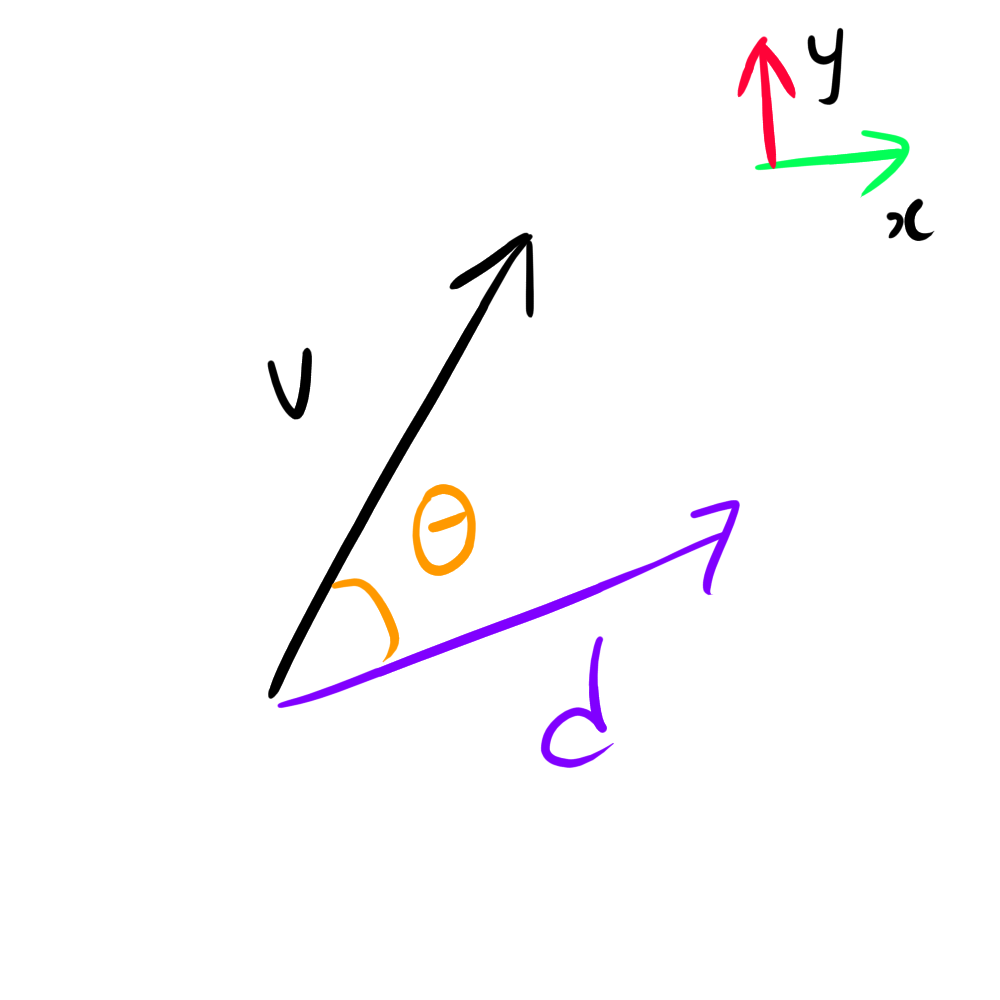
\includegraphics[width=0.3\textwidth,right]{assets/angular_freedom.png}
    \caption{Angular function}
    \label{fig:angular_freedom}
\end{figure}

Define the player's direction in terms of the smallest angle between unit directional vector $\td(t)$ and the velocity $\tv(t)$, denoted as $\theta(t)$ as a function of time (figure \ref{fig:angular_freedom}). This function's domain is limited between $0$ and $\pi$ par definition. Therefore the directional vector is the player's unit velocity rotated by angle $\theta$
\[
    \td(t) = \exp((\phi(t) - \theta(t)) \I).
\]


%\begin{wrapfigure}{r}{0.40\textwidth}
%    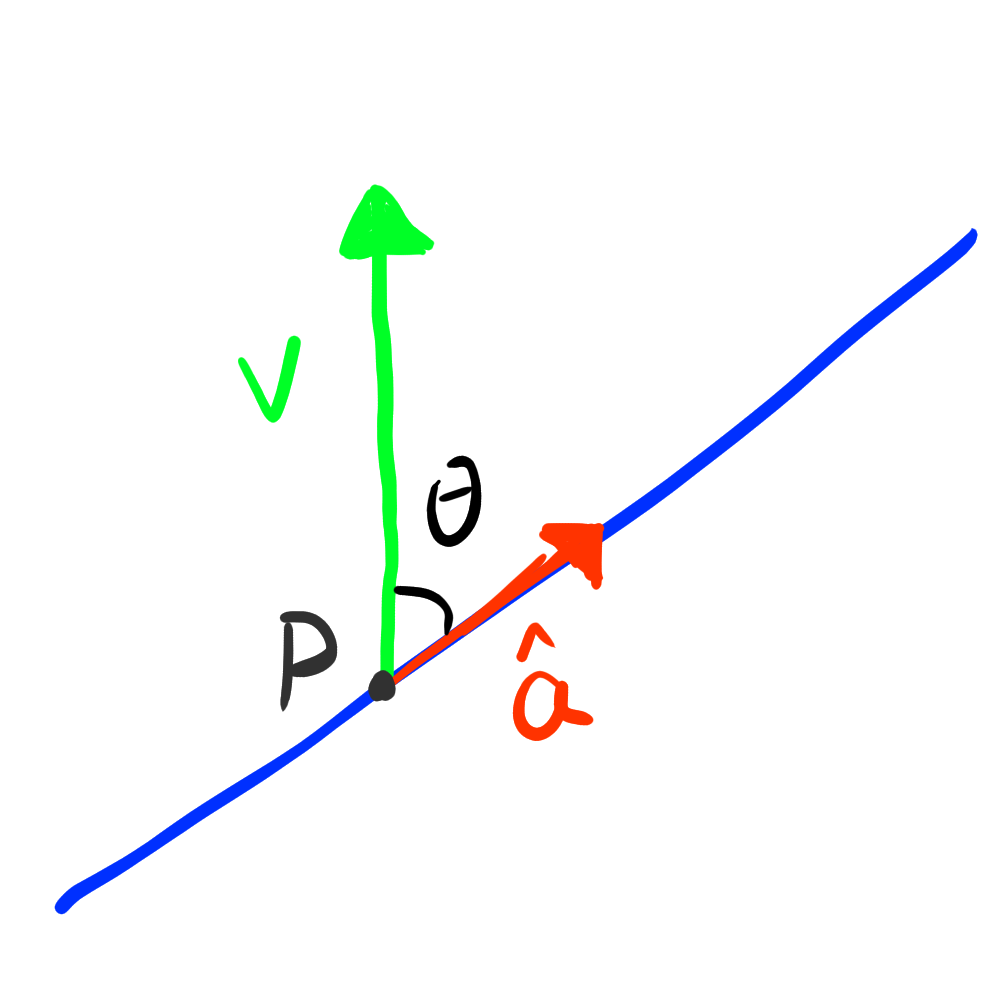
\includegraphics[width=0.37\textwidth,right]{assets/angular.png}
%    \caption{The angular function}
%    \label{fig:angular}
%\end{wrapfigure}
%
%Using the discrete updating formulas in Eq.\ref{eq:1de1}, Eq.\ref{eq:1de2} and the piecewise acceleration function in figure \ref{eq:playeracceleration}, the velocity update can be rewritten in the angular form:
%\begin{align*}
%    \tv' &= \tv + LA \exp((\phi - \theta) \I),
%\end{align*}
%with assumption that $\ta$ is maximized. Also, the position update remains unchanged:
%\[
%    \tp' = \tp + \tau \tv.
%\]
It is now possible to rewrite the speed limit as a simple cosine inequality. Because $\td(t)$ and $\tv(t)$ are two dimensional, the dot product identity yields
\begin{align*}
    \text{proj}(\td, \tv) &= \td \cdot \tv\\
    &= \tmag{\td} \tmag{\tv} \cos \theta\\
    &= r \cos \theta.
\end{align*}


%In order to maximize jumping displacement, it seems reasonable to maximize velocity and therefore maximize acceleration. This means to maximize the scalar $w$, which is equivalent to finding a function that fits the constraint in equation \ref{eq:constraint}.

%Remember that the scalar function $w$ is defined piecewise:
%\[
%    w = \begin{cases}
%        \gamma_1 & \gamma_2 \ge \gamma_1\\
%     \gamma_2 & \gamma_1 > \gamma_2 > 0\\
%     0 & 0 \ge \gamma_2
%    \end{cases},
%\]
%where $\gamma_1 = LA\tau$ and $\gamma_2 = L - \tv \cdot \tunit{a}$. This can be rewritten in terms of our new angular function $\theta(t)$.
\begin{figure}[H]
    %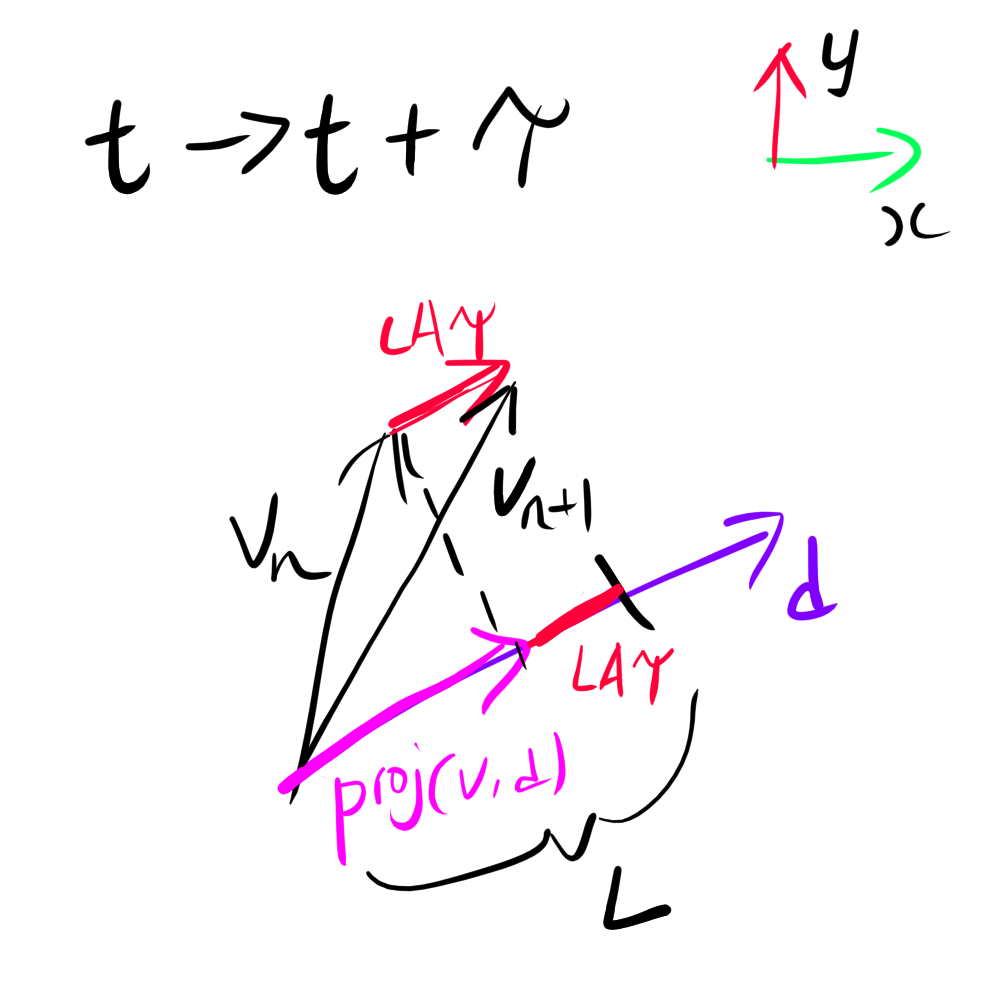
\includegraphics[width=0.37\textwidth,right]{assets/discrete_limit.png}
    \centering
    \sized[0.4]{


\tikzset{every picture/.style={line width=0.75pt}} %set default line width to 0.75pt

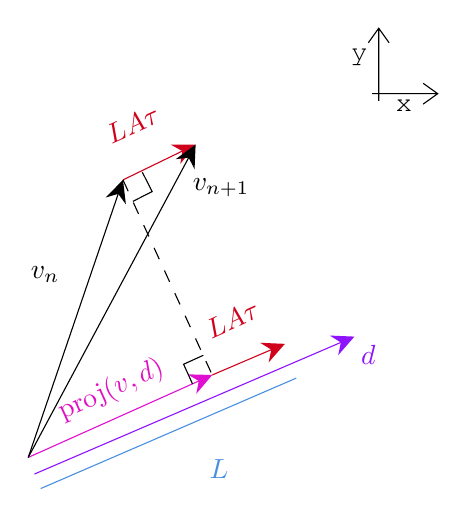
\begin{tikzpicture}[x=0.75pt,y=0.75pt,yscale=-1,xscale=1]
%uncomment if require: \path (0,269); %set diagram left start at 0, and has height of 269

%Shape: Axis 2D [id:dp3688296019635018]
\draw [color={rgb, 255:red, 0; green, 0; blue, 0 }  ,draw opacity=1 ] (419.68,43.2) -- (451.25,43.2)(422.84,11.66) -- (422.84,46.7) (444.25,38.2) -- (451.25,43.2) -- (444.25,48.2) (417.84,18.66) -- (422.84,11.66) -- (427.84,18.66)  ;
%Straight Lines [id:da15946190790496706]
\draw [color={rgb, 255:red, 224; green, 16; blue, 209 }  ,draw opacity=1 ]   (253.98,218.45) -- (339.9,179.96) ;
\draw [shift={(342.63,178.73)}, rotate = 155.87] [fill={rgb, 255:red, 224; green, 16; blue, 209 }  ,fill opacity=1 ][line width=0.08]  [draw opacity=0] (10.72,-5.15) -- (0,0) -- (10.72,5.15) -- (7.12,0) -- cycle    ;
%Straight Lines [id:da23789994899521405]
\draw    (253.98,218.45) -- (298.66,87.57) ;
\draw [shift={(299.63,84.73)}, rotate = 108.85] [fill={rgb, 255:red, 0; green, 0; blue, 0 }  ][line width=0.08]  [draw opacity=0] (10.72,-5.15) -- (0,0) -- (10.72,5.15) -- (7.12,0) -- cycle    ;
%Straight Lines [id:da7945400962055216]
\draw [color={rgb, 255:red, 208; green, 2; blue, 27 }  ,draw opacity=1 ]   (299.63,84.73) -- (317.53,76.04) -- (331.93,69.04) ;
\draw [shift={(334.63,67.73)}, rotate = 154.09] [fill={rgb, 255:red, 208; green, 2; blue, 27 }  ,fill opacity=1 ][line width=0.08]  [draw opacity=0] (10.72,-5.15) -- (0,0) -- (10.72,5.15) -- (7.12,0) -- cycle    ;
%Straight Lines [id:da32752633260821995]
\draw  [dash pattern={on 4.5pt off 4.5pt}]  (299.63,84.73) -- (309.1,105.43) -- (342.63,178.73) ;
%Shape: Right Angle [id:dp1944206914820521]
\draw   (333.14,183.05) -- (328.83,173.55) -- (338.32,169.24) ;
%Straight Lines [id:da11716809450724408]
\draw    (253.98,218.45) -- (333.22,70.38) ;
\draw [shift={(334.63,67.73)}, rotate = 118.15] [fill={rgb, 255:red, 0; green, 0; blue, 0 }  ][line width=0.08]  [draw opacity=0] (10.72,-5.15) -- (0,0) -- (10.72,5.15) -- (7.12,0) -- cycle    ;
%Shape: Right Angle [id:dp26249838064168163]
\draw   (308.97,81.07) -- (313.67,90.38) -- (304.37,95.08) ;
%Straight Lines [id:da3181116090278877]
\draw [color={rgb, 255:red, 208; green, 2; blue, 27 }  ,draw opacity=1 ]   (342.63,178.73) -- (374.88,164.92) ;
\draw [shift={(377.63,163.73)}, rotate = 156.8] [fill={rgb, 255:red, 208; green, 2; blue, 27 }  ,fill opacity=1 ][line width=0.08]  [draw opacity=0] (10.72,-5.15) -- (0,0) -- (10.72,5.15) -- (7.12,0) -- cycle    ;
%Straight Lines [id:da11758138251143024]
\draw [color={rgb, 255:red, 144; green, 19; blue, 254 }  ,draw opacity=1 ]   (256.98,226.45) -- (408.38,161.42) ;
\draw [shift={(411.13,160.23)}, rotate = 156.75] [fill={rgb, 255:red, 144; green, 19; blue, 254 }  ,fill opacity=1 ][line width=0.08]  [draw opacity=0] (10.72,-5.15) -- (0,0) -- (10.72,5.15) -- (7.12,0) -- cycle    ;
%Straight Lines [id:da7832053208510404]
\draw [color={rgb, 255:red, 74; green, 144; blue, 226 }  ,draw opacity=1 ]   (259.98,233.45) -- (383.13,180.23) ;

% Text Node
\draw (429.67,44.67) node [anchor=north west][inner sep=0.75pt]   [align=left] {{\fontfamily{pcr}\selectfont x}};
% Text Node
\draw (408.33,20) node [anchor=north west][inner sep=0.75pt]   [align=left] {{\fontfamily{pcr}\selectfont y}};
% Text Node
\draw (253.98,125) node [anchor=north west][inner sep=0.75pt]   [align=left] {$\displaystyle v_{n}$};
% Text Node
\draw (331.98,83) node [anchor=north west][inner sep=0.75pt]   [align=left] {$\displaystyle v_{n+1}$};
% Text Node
\draw (336.74,152.6) node [anchor=north west][inner sep=0.75pt]  [color={rgb, 255:red, 208; green, 2; blue, 27 }  ,opacity=1 ,rotate=-335.67] [align=left] {$\displaystyle LA\tau $};
% Text Node
\draw (264.74,190.6) node [anchor=north west][inner sep=0.75pt]  [color={rgb, 255:red, 224; green, 16; blue, 194 }  ,opacity=1 ,rotate=-335.67] [align=left] {proj$\displaystyle ( v,d)$};
% Text Node
\draw (288.74,58.6) node [anchor=north west][inner sep=0.75pt]  [color={rgb, 255:red, 208; green, 2; blue, 27 }  ,opacity=1 ,rotate=-335.67] [align=left] {$\displaystyle LA\tau $};
% Text Node
\draw (413.13,163.23) node [anchor=north west][inner sep=0.75pt]  [color={rgb, 255:red, 144; green, 19; blue, 254 }  ,opacity=1 ] [align=left] {$\displaystyle d$};
% Text Node
\draw (340.06,218.34) node [anchor=north west][inner sep=0.75pt]  [color={rgb, 255:red, 74; green, 144; blue, 226 }  ,opacity=1 ] [align=left] {$\displaystyle L$};


\end{tikzpicture}

    }
    \caption{Discrete frame and limit}
    \label{fig:discrete_limit}
\end{figure}

Also the entire inequality will be different in the discrete case. Not only does the projection $\text{proj}(\td, \tv)$ has to be less than the speed limit, but it also has to allow the maximum discrete acceleration of magnitude $LA\tau$ every frame (figure \ref{fig:discrete_limit}).

Therefore, the inequality condition must be rewritten discretely: (Because cosine is a decreasing function, the inequality sign must be reversed \citefoot{ineqcosine})
\begin{align*}
    L &\ge \text{proj}(\td, \tv) + LA\tau\\
    L - LA\tau &\ge \text{proj}(\td, \tv)\\
    &\ge r \cos \theta,\\
    \frac{L - LA\tau}{r} &\ge \cos \theta\\
    \cos^{-1} (\frac{L - LA\tau}{r}) &\le \theta.
\end{align*}

\begin{figure}[H]
    \centering
    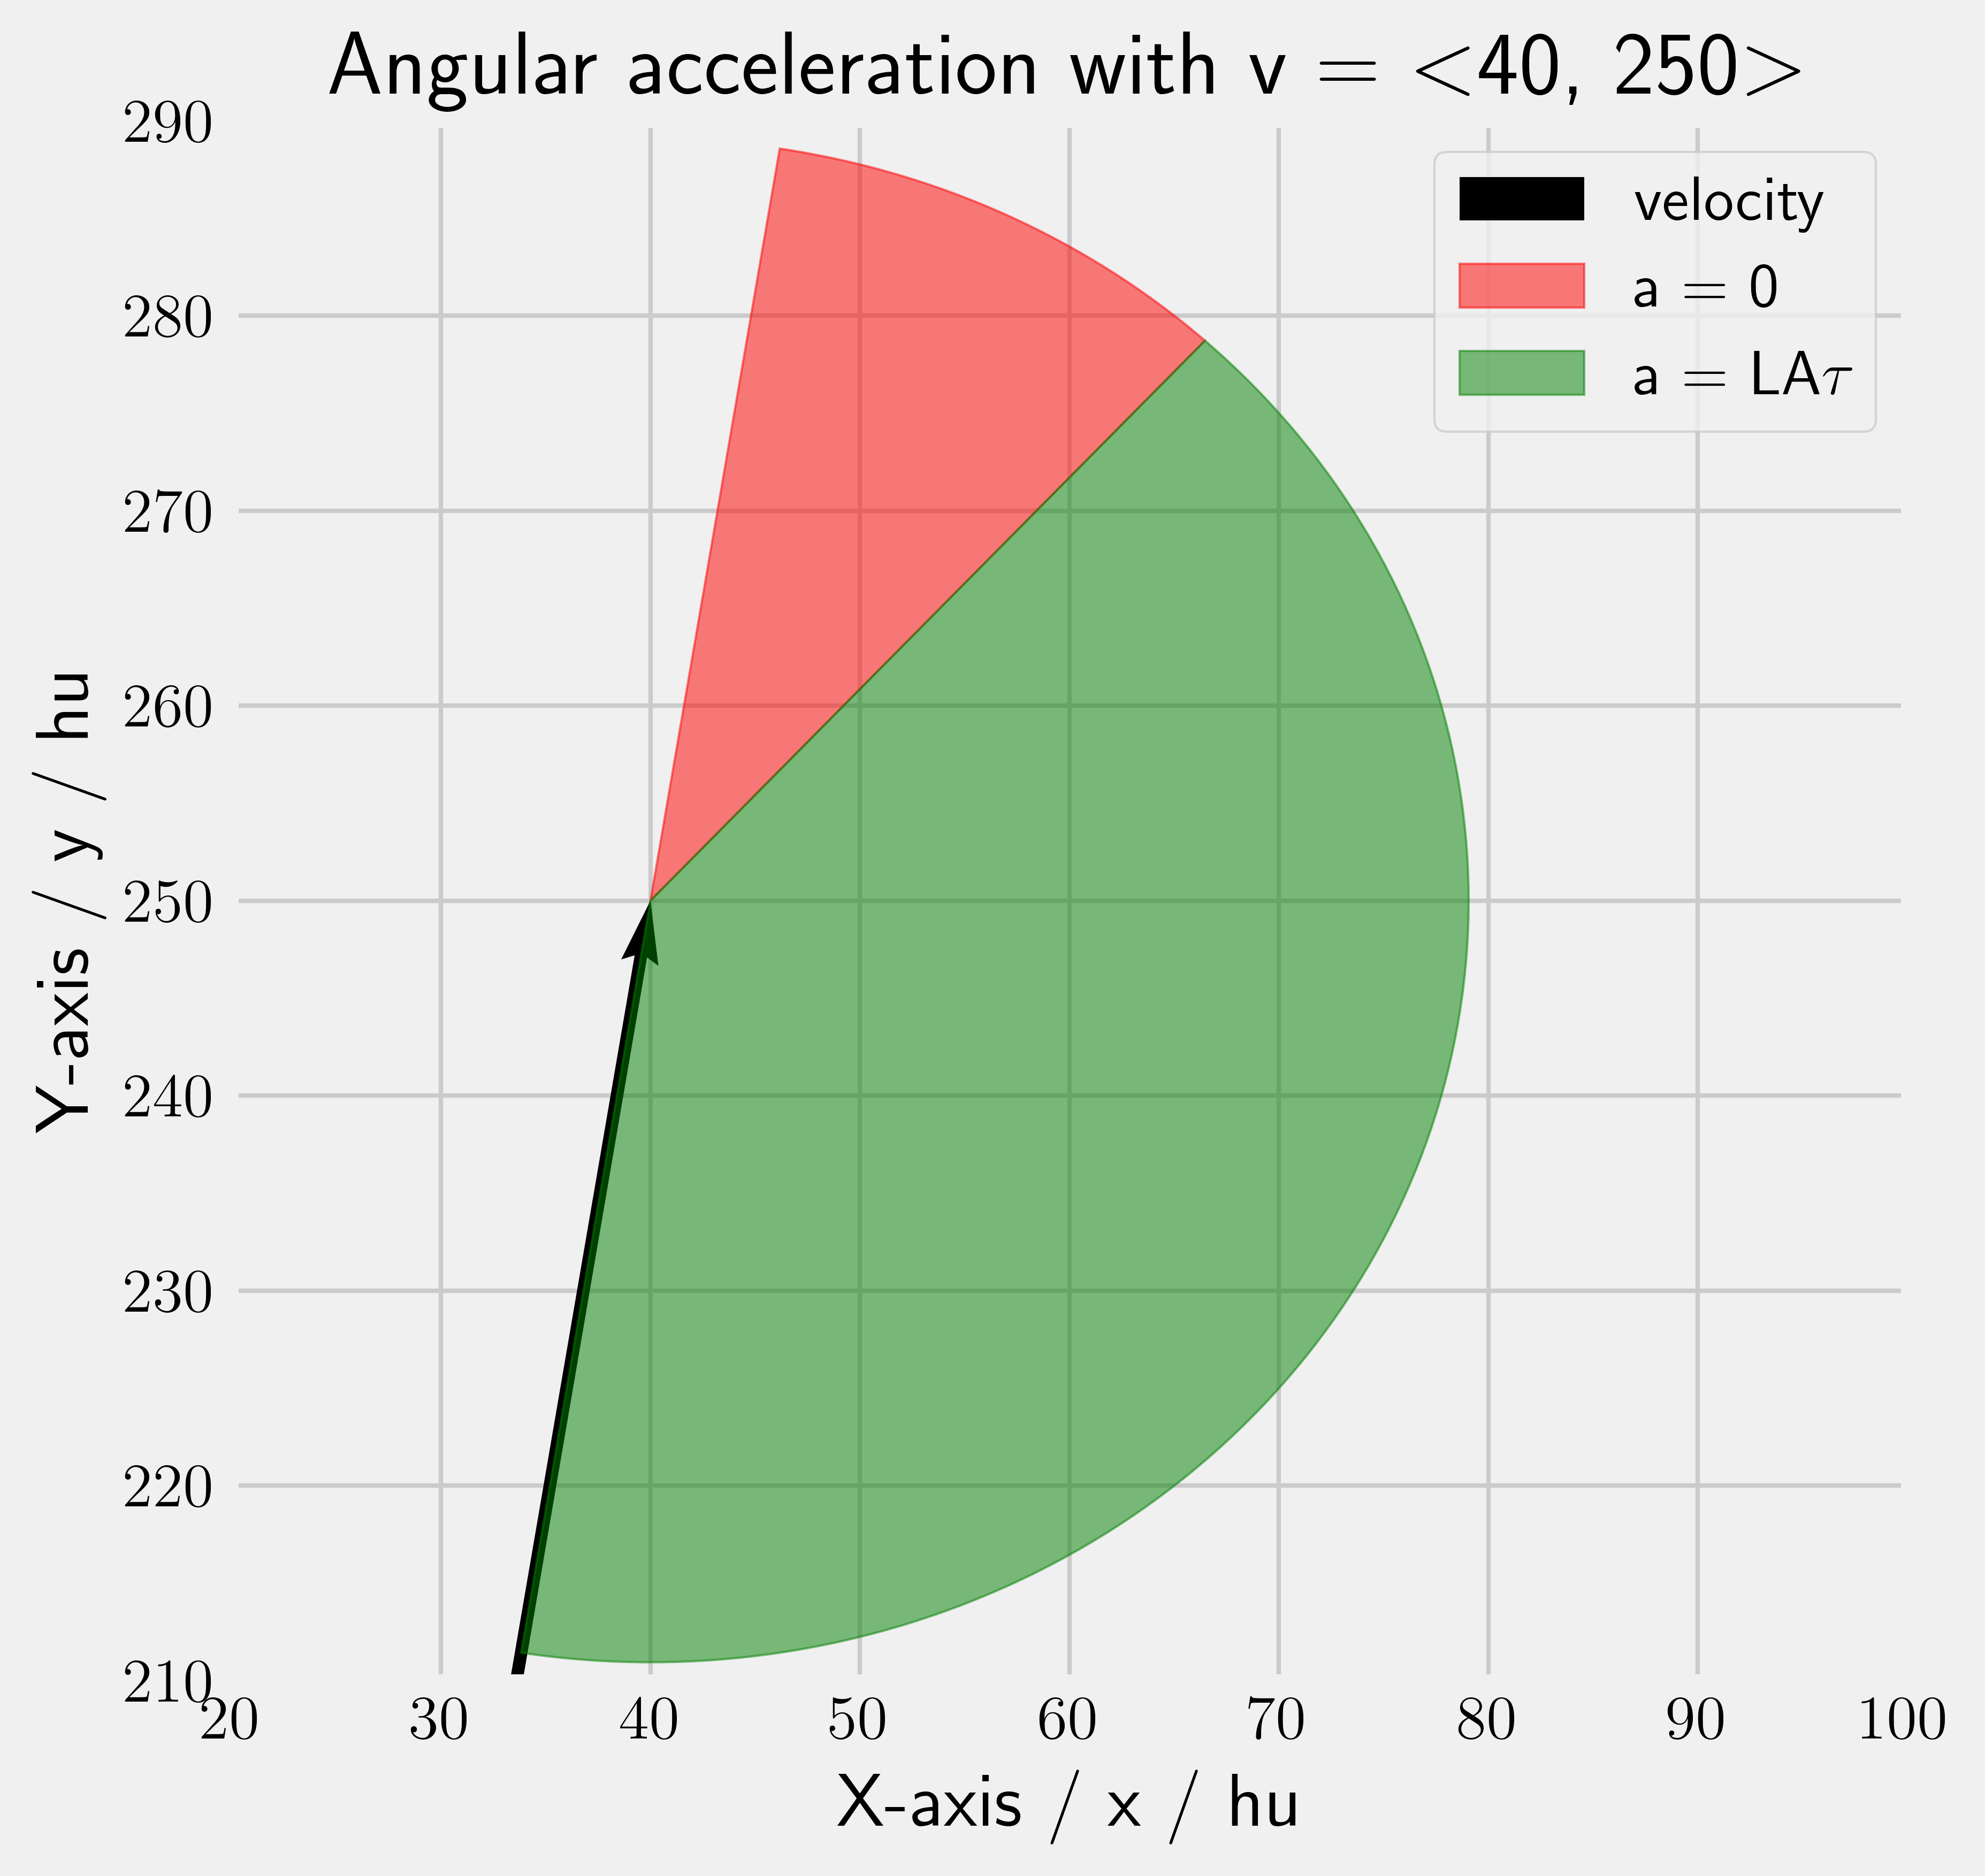
\includegraphics[width=0.5\textwidth]{assets/angular_acceleration_limiting.png}
    \caption{Angular acceleration}
    \label{fig:angular_acceleration_limiting}
\end{figure}

The equation shows that $\theta(t)$ must be greater or equal to a value for maximum acceleration. Figure \ref{fig:angular_acceleration_limiting} demonstrates the magnitude of acceleration for all angles of $\theta$ under a player velocity of $\tang{40, 250}$. The red area indicates zero acceleration, because the small $\theta$ exceeds the speed limit; the green area means full acceleration, so larger $\theta$ or more rotation of $\td$ against $\tv$ will result in higher acceleration.

Therefore, we can rewrite the planer acceleration function $\ta(t)$ with:
\[
\ta(t) = \begin{cases}
    LA & \cos^{-1}(\frac{L - LA\tau}{r}) \leq \theta\\
    0 & \cos^{-1}(\frac{L - LA\tau}{r}) > \theta
\end{cases}
\]


\subsubsection{Optimization}
%Using the same argument as the straight-line model, I will use an initial velocity of $\tv_0 = \tang{0, 250}$.
To maximize acceleration at each frame, I noticed that the player would want to minimize $\theta(t)$. This is due to the the law of cosine\citefoot{lawofcosine} (figure \ref{fig:min_theta}).

\begin{figure}[H]
    \centering
    %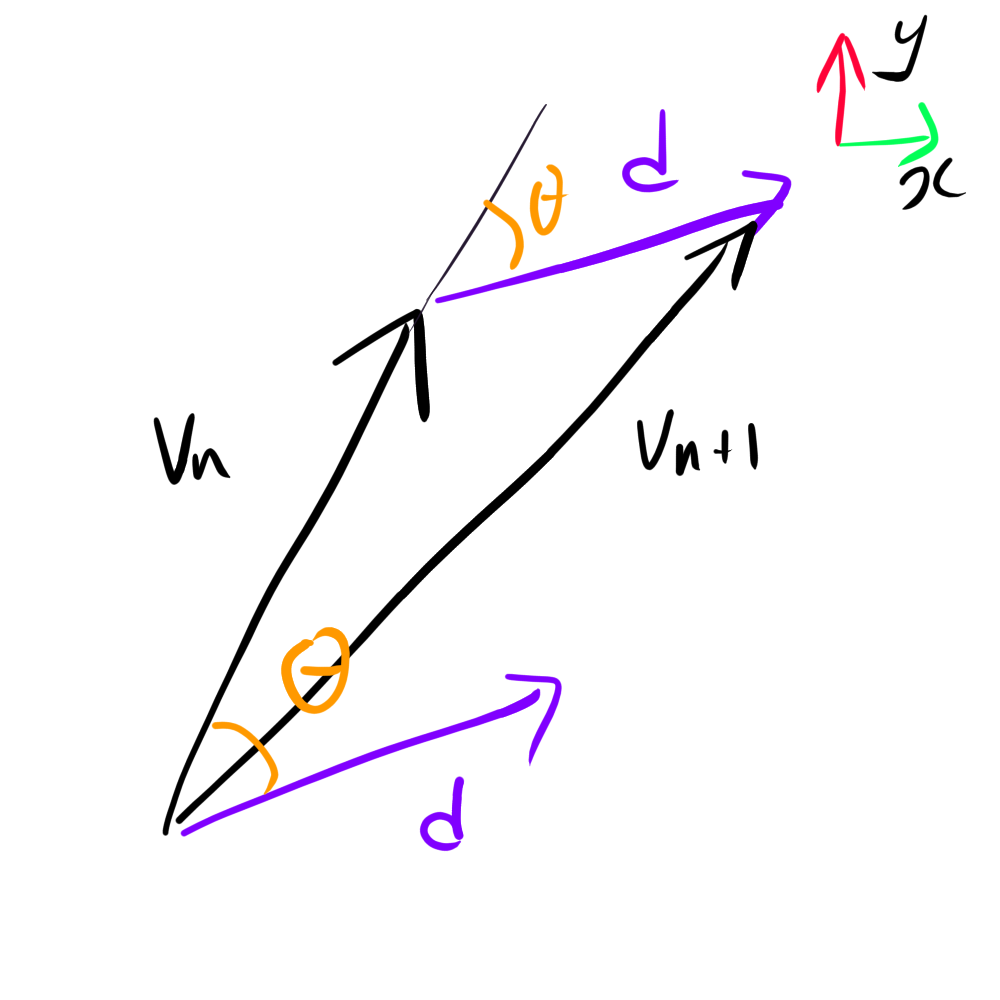
\includegraphics[width=0.37\textwidth,right]{assets/mini_theta.png}
    \sized{


\tikzset{every picture/.style={line width=0.75pt}} %set default line width to 0.75pt

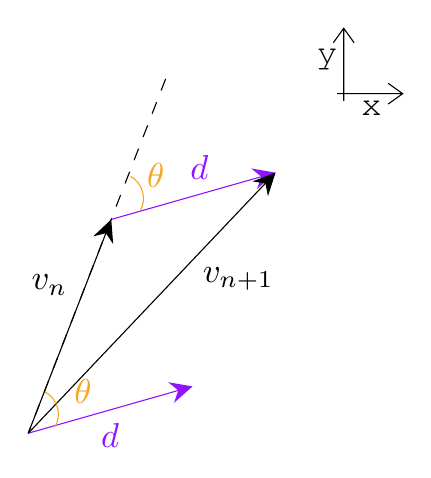
\begin{tikzpicture}[x=0.75pt,y=0.75pt,yscale=-1,xscale=1]
%uncomment if require: \path (0,300); %set diagram left start at 0, and has height of 300

%Shape: Axis 2D [id:dp161788656784575]
\draw [color={rgb, 255:red, 0; green, 0; blue, 0 }  ,draw opacity=1 ] (443.68,70.2) -- (475.25,70.2)(446.84,38.66) -- (446.84,73.7) (468.25,65.2) -- (475.25,70.2) -- (468.25,75.2) (441.84,45.66) -- (446.84,38.66) -- (451.84,45.66)  ;
%Straight Lines [id:da6082790355416728]
\draw [color={rgb, 255:red, 144; green, 19; blue, 254 }  ,draw opacity=1 ]   (294.85,233.78) -- (371.11,212.06) ;
\draw [shift={(374,211.23)}, rotate = 164.1] [fill={rgb, 255:red, 144; green, 19; blue, 254 }  ,fill opacity=1 ][line width=0.08]  [draw opacity=0] (10.72,-5.15) -- (0,0) -- (10.72,5.15) -- (7.12,0) -- cycle    ;
%Straight Lines [id:da529580686828609]
\draw [color={rgb, 255:red, 144; green, 19; blue, 254 }  ,draw opacity=1 ]   (334.85,130.78) -- (411.11,109.06) ;
\draw [shift={(414,108.23)}, rotate = 164.1] [fill={rgb, 255:red, 144; green, 19; blue, 254 }  ,fill opacity=1 ][line width=0.08]  [draw opacity=0] (10.72,-5.15) -- (0,0) -- (10.72,5.15) -- (7.12,0) -- cycle    ;
%Straight Lines [id:da6869395653145243]
\draw    (294.85,233.78) -- (333.76,133.58) ;
\draw [shift={(334.85,130.78)}, rotate = 111.22] [fill={rgb, 255:red, 0; green, 0; blue, 0 }  ][line width=0.08]  [draw opacity=0] (10.72,-5.15) -- (0,0) -- (10.72,5.15) -- (7.12,0) -- cycle    ;
%Straight Lines [id:da8505569385359156]
\draw    (294.85,233.78) -- (411.93,110.41) ;
\draw [shift={(414,108.23)}, rotate = 133.5] [fill={rgb, 255:red, 0; green, 0; blue, 0 }  ][line width=0.08]  [draw opacity=0] (10.72,-5.15) -- (0,0) -- (10.72,5.15) -- (7.12,0) -- cycle    ;
%Shape: Arc [id:dp13917835626195973]
\draw  [draw opacity=0] (303.12,213.99) .. controls (306.02,215.62) and (308.25,218.41) .. (309.06,221.91) .. controls (309.76,224.95) and (309.25,227.98) .. (307.86,230.51) -- (297.17,224.64) -- cycle ; \draw  [color={rgb, 255:red, 245; green, 166; blue, 35 }  ,draw opacity=1 ] (303.12,213.99) .. controls (306.02,215.62) and (308.25,218.41) .. (309.06,221.91) .. controls (309.76,224.95) and (309.25,227.98) .. (307.86,230.51) ;
%Straight Lines [id:da505532385848832]
\draw  [dash pattern={on 4.5pt off 4.5pt}]  (361.05,63.07) -- (294.85,233.78) ;
%Shape: Arc [id:dp87688867176111]
\draw  [draw opacity=0] (344.12,109.99) .. controls (347.02,111.62) and (349.25,114.41) .. (350.06,117.91) .. controls (350.76,120.95) and (350.25,123.98) .. (348.86,126.51) -- (338.17,120.64) -- cycle ; \draw  [color={rgb, 255:red, 245; green, 166; blue, 35 }  ,draw opacity=1 ] (344.12,109.99) .. controls (347.02,111.62) and (349.25,114.41) .. (350.06,117.91) .. controls (350.76,120.95) and (350.25,123.98) .. (348.86,126.51) ;

% Text Node
\draw (453.67,71.67) node [anchor=north west][inner sep=0.75pt]  [xscale=1.25,yscale=1.25] [align=left] {{\fontfamily{pcr}\selectfont x}};
% Text Node
\draw (432.33,47) node [anchor=north west][inner sep=0.75pt]  [xscale=1.25,yscale=1.25] [align=left] {{\fontfamily{pcr}\selectfont y}};
% Text Node
\draw (315.52,206.4) node [anchor=north west][inner sep=0.75pt]  [color={rgb, 255:red, 245; green, 166; blue, 35 }  ,opacity=1 ,xscale=1.25,yscale=1.25] [align=left] {$\displaystyle \theta $};
% Text Node
\draw (350.52,102.4) node [anchor=north west][inner sep=0.75pt]  [color={rgb, 255:red, 245; green, 166; blue, 35 }  ,opacity=1 ,xscale=1.25,yscale=1.25] [align=left] {$\displaystyle \theta $};
% Text Node
\draw (294.85,156) node [anchor=north west][inner sep=0.75pt]  [xscale=1.25,yscale=1.25] [align=left] {$\displaystyle v_{n}$};
% Text Node
\draw (377.43,152.51) node [anchor=north west][inner sep=0.75pt]  [xscale=1.25,yscale=1.25] [align=left] {$\displaystyle v_{n+1}$};
% Text Node
\draw (328.43,227.51) node [anchor=north west][inner sep=0.75pt]  [color={rgb, 255:red, 144; green, 19; blue, 254 }  ,opacity=1 ,xscale=1.25,yscale=1.25] [align=left] {$\displaystyle d$};
% Text Node
\draw (371.43,98.51) node [anchor=north west][inner sep=0.75pt]  [color={rgb, 255:red, 144; green, 19; blue, 254 }  ,opacity=1 ,xscale=1.25,yscale=1.25] [align=left] {$\displaystyle d$};


\end{tikzpicture}

    }
    \caption{Minimizing $\theta(t)$}
    \label{fig:min_theta}
\end{figure}

Let $v_n = \tmag{\tv_n}$, $v_{n+1} = \tmag{\tv_{n+1}}$, and $d = \tmag{d}$. The length of the updated velocity $v_{n+1}$ using the law of cosine on the opposite angle of $\theta(t)$ is
\[
    v_{n+1} = \sqrt{v_n^2 + d_n^2 - 2 v_n d\cos (\pi - \theta(t))}.
\]
Because only $\theta$ is controlled by the player, to maximize the updated velocity $v_{n+1}$ means minimizing $\cos(\pi - \theta(t))$. For the cosine function is smaller at higher $x$ values, we need to maximize $\pi - \theta(t)$ and therefore minimize $\theta(t)$.

Therefore for maximum acceleration, the player needs to minimize $\theta(t)$ while keeping it above a value. This means that we should set $\theta(t)$ to equal the value at all times, so
\[
    \theta(t) = \cos^{-1} \left( \frac{L-LA\tau}{r} \right).
\]

Notice that $\theta(t)$ increases as the magnitude of velocity increases over time, which agrees with the skilled player's theory of turning overtime. However, this means that the acceleration will decrease over time as well.

By substituting this equation of $\theta(t)$ into the difference equation of Eq.\ref{eq:1de1}, I derived the difference equation for my first discrete model:
\begin{figure}[H]
    \centering
    \[
        \tv_{n+1} = LA\tau \exp\left(\left(\phi - \cos^{-1}\left(\frac{L-LA\tau}{r}\right)\right) \I\right).
    \]
    \caption{First discrete difference equation}
    \label{fig:sbs}
\end{figure}

Figure \ref{fig:1sbs} shows the player's motion under this method.

\begin{figure}[H]
    \centering
    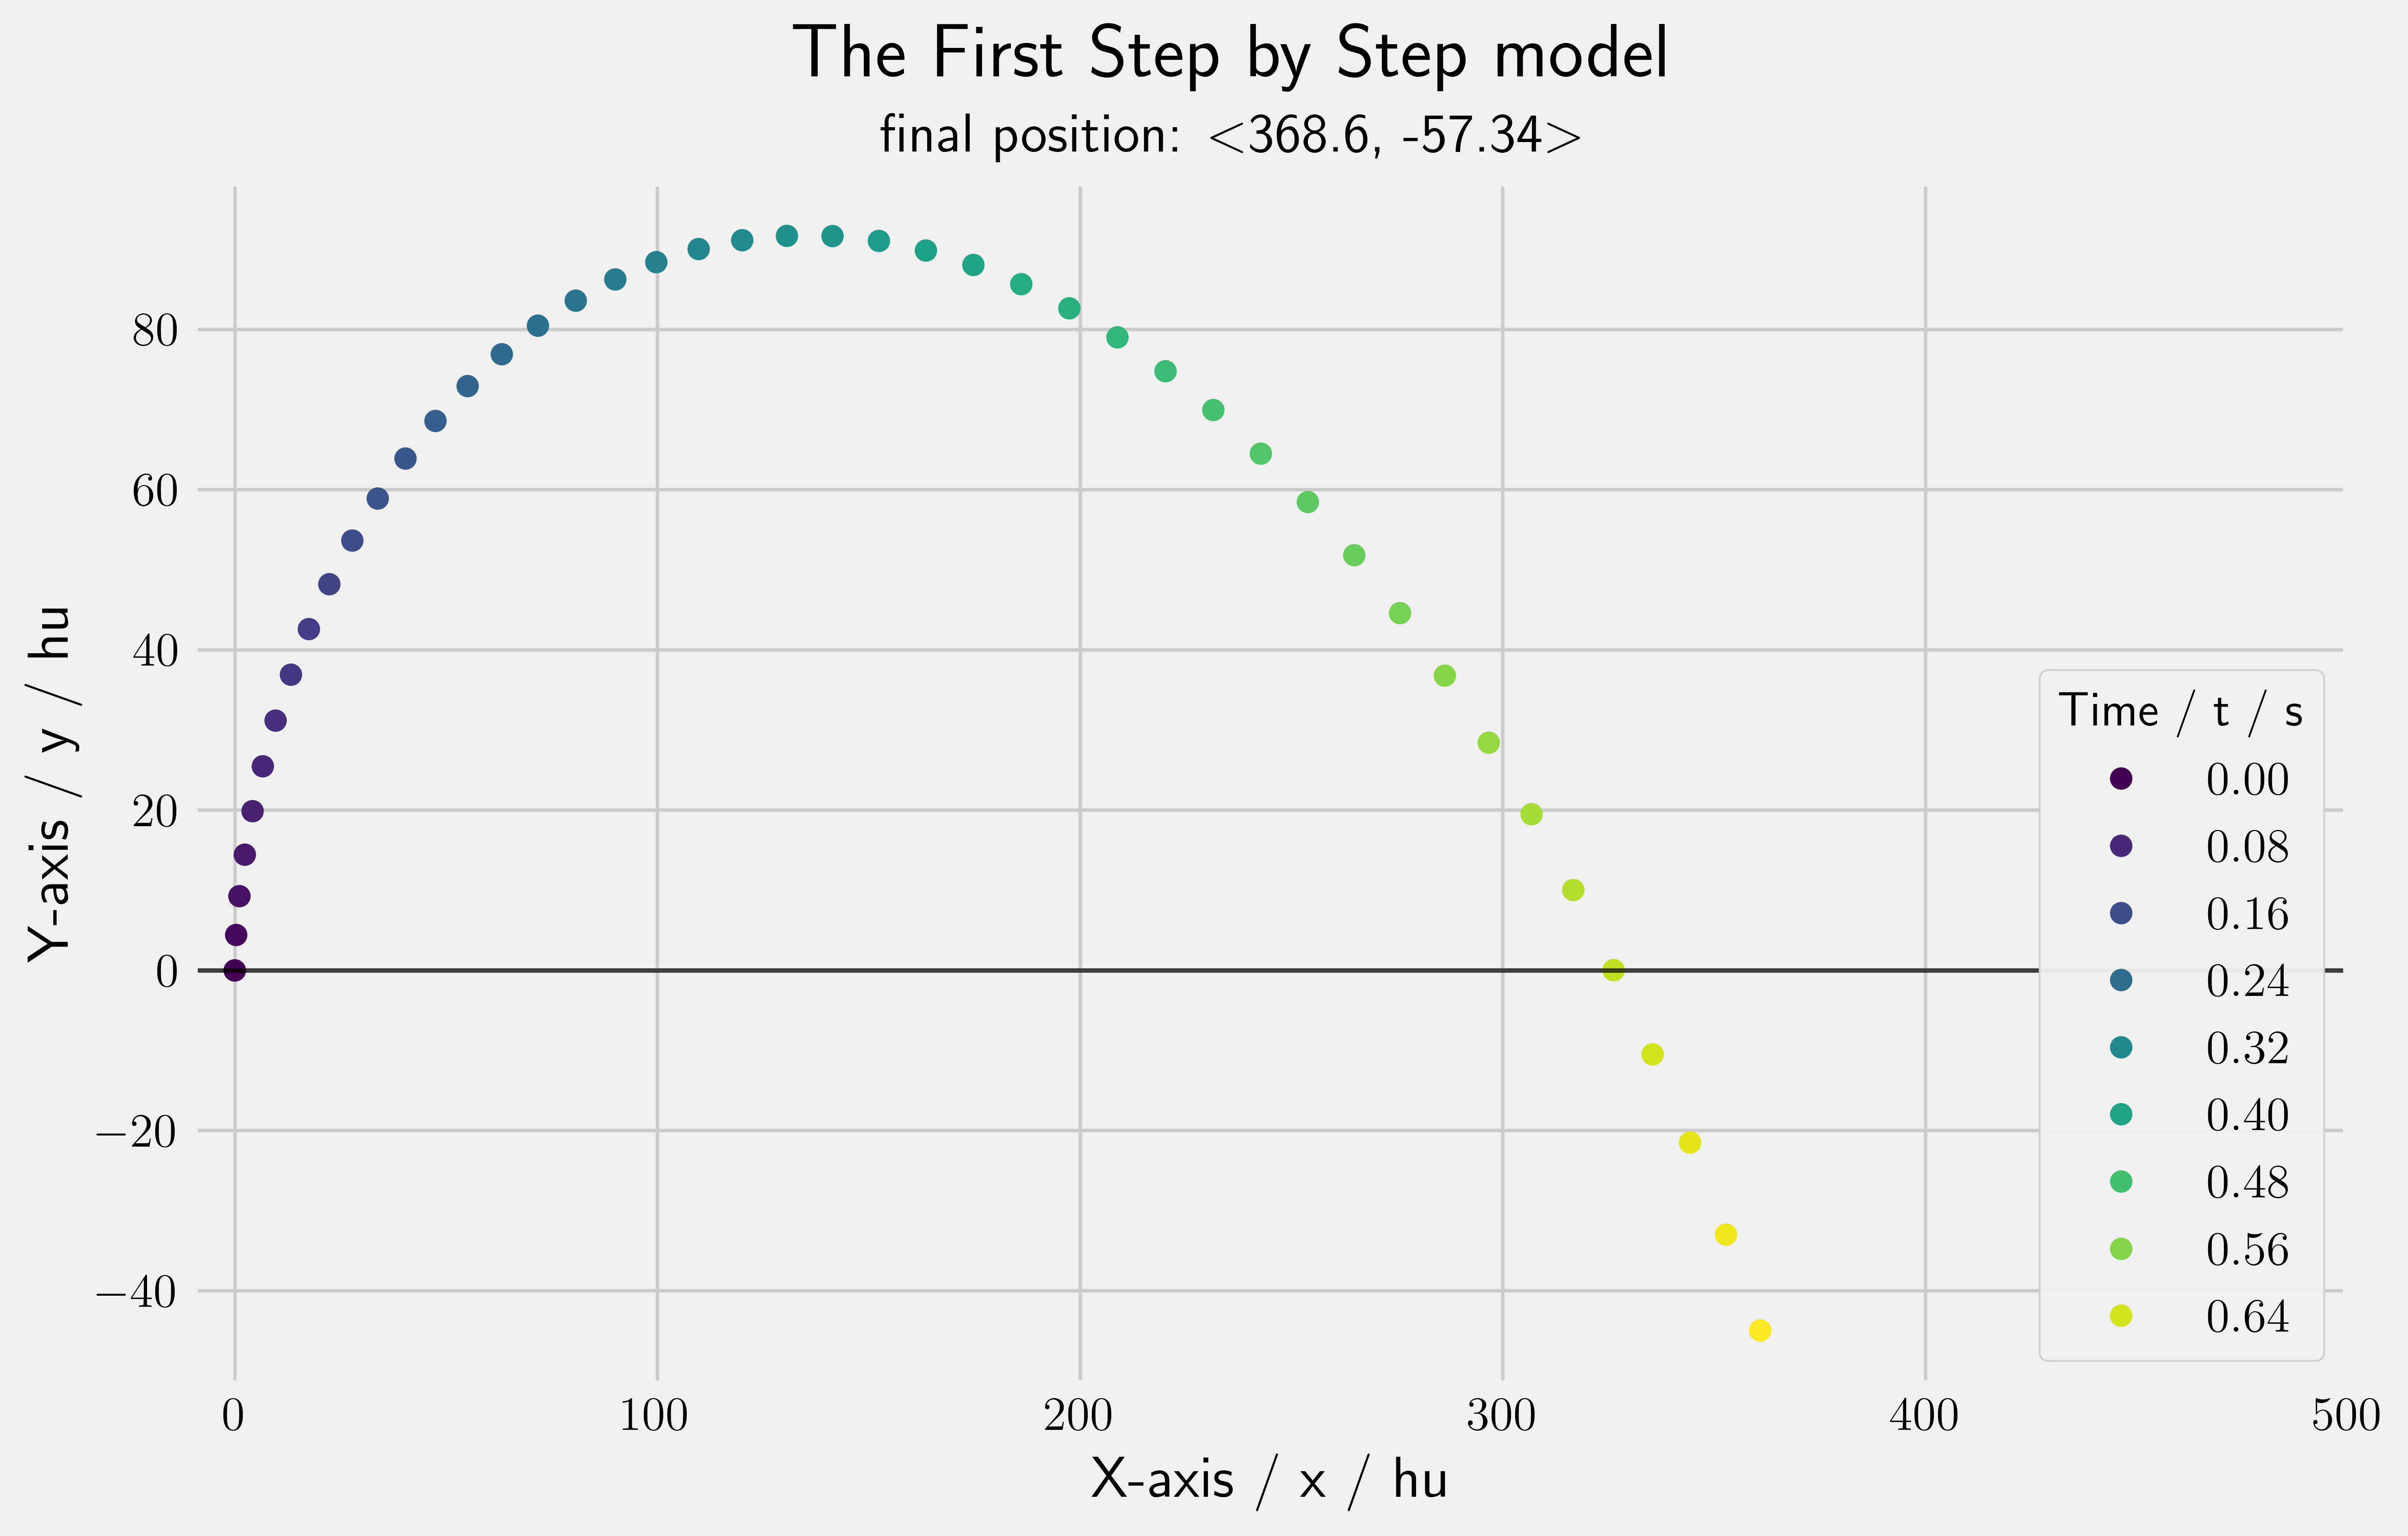
\includegraphics[width=0.8\textwidth]{assets/step_by_step_1.png}
    \caption{}
    \label{fig:1sbs}
\end{figure}

It seems like the player completed a u-turn and ended up below the x-axis. Although the distance between each position dots are increasing indicating acceleration, this strategy had to keep turning to maximize that, which may reduced our displacement at a certain angle. Nevertheless, this model created a displacement of $\sqrt{368.6^2 + (-57.34)^2} \approx 373.0$, which is a large increase from the previous models.

\subsection{Discrete model with modification}
The first discrete model (figure \ref{fig:1sbs}) had a problem, which is that the player needed to keep turning to maximize acceleration. I have an idea to fix it: stop turning at an angle.

The arguments for stop turning is that we are sacrificing potential higher velocity and less distance traveled but directing more outwards movement that could increase the total displacement. Moreover, the success of this modification could disprove my conjunctures stating that higher acceleration leads to higher velocity, and therefore higher displacement.

So let there be a maximum angle $k$ for player velocity, which once reached would set $\theta(t) = 0$. We can represent this modification as a piecewise function named the second discrete difference equation:

\begin{figure}[H]
    \centering
    \[
        \tv_{n+1} = \begin{cases}
            LA\tau \exp\left(\left(\phi - \cos^{-1}\left(\frac{L-LA\tau}{r}\right)\right) \I\right) & \phi < k\\
            0 & \phi \geq k
        \end{cases}
    \]
    \caption{Second discrete difference equation}
    \label{fig:ssbs}
\end{figure}



\begin{figure}[H]
    \centering
    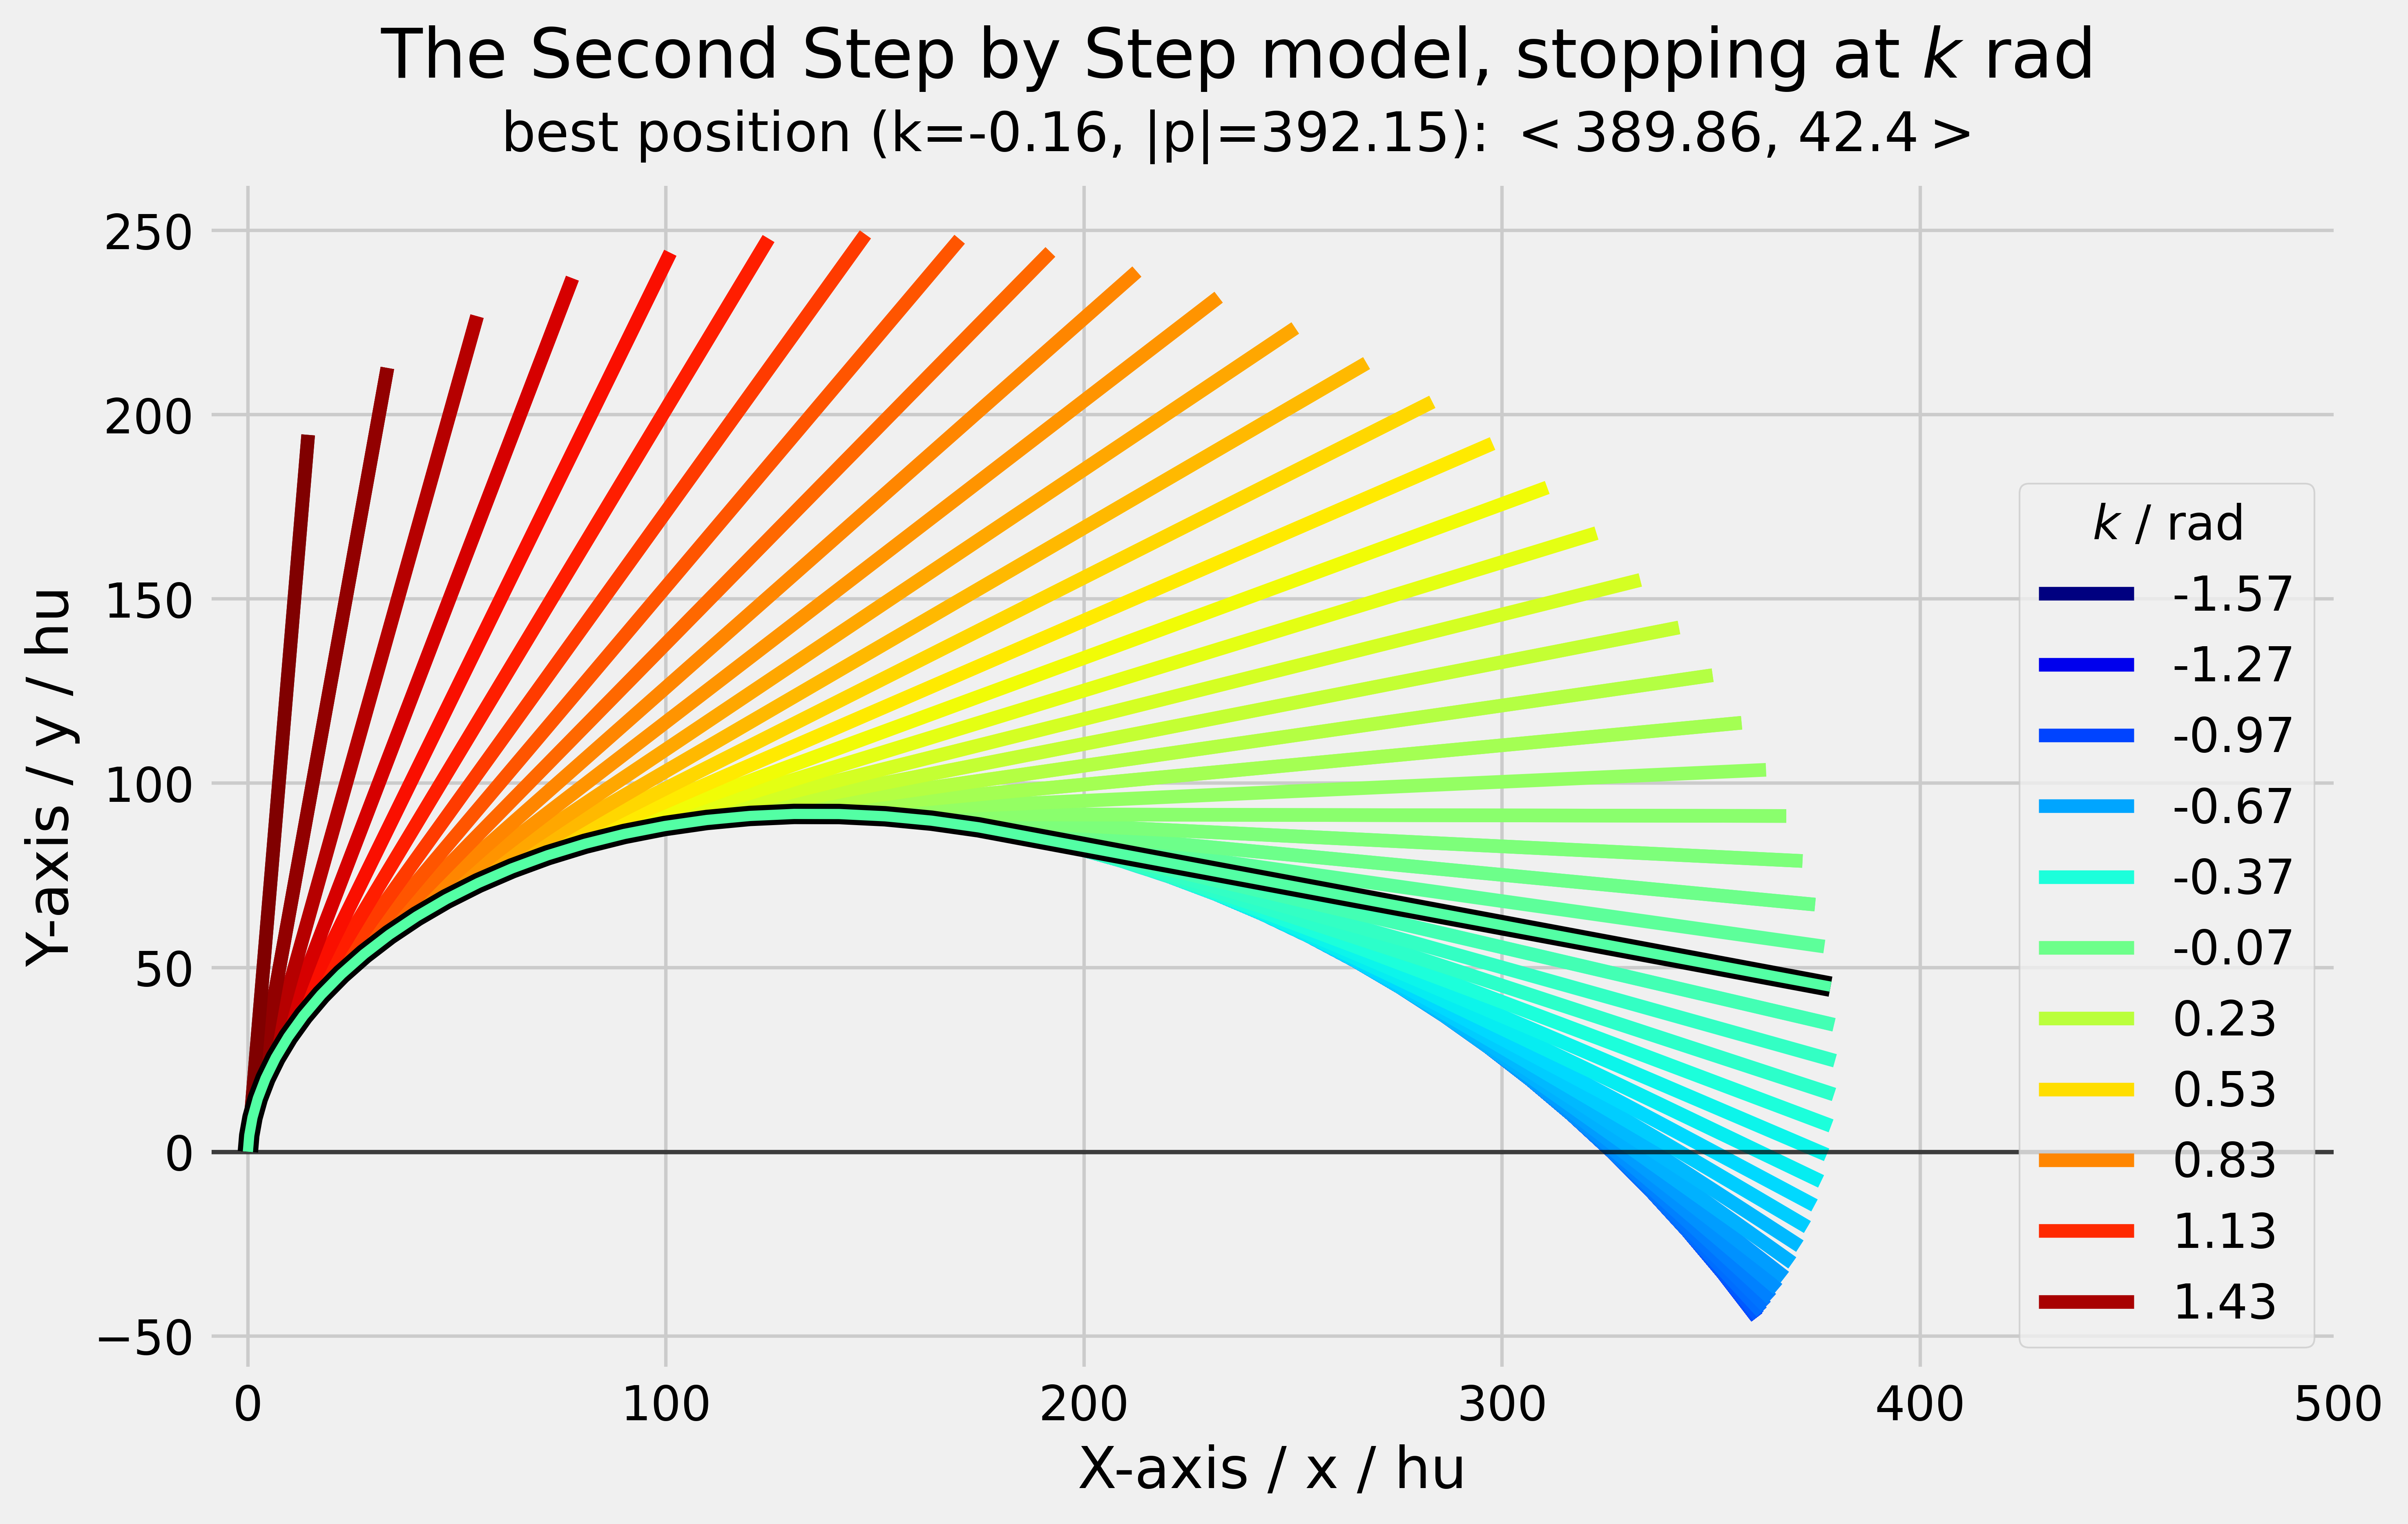
\includegraphics[width=0.8\textwidth]{assets/step_by_step_2.png}
    \caption{}
    \label{fig:sbs2}
\end{figure}

Figure \ref{fig:sbs2} shows the different player motion as the maximum angle $k\in [-0.5\pi, 0.5\pi]$ with $0.03$ radians steps for clarity. The paths of maximum displacement is outlined in black, with displacement $\approx 392.15$ at $k=-0.16$. As expected, the total turning of the player decreased at the most optimal path. The value $k$ is slightly below $0$, meaning that it is still beneficial --- at least for a bit --- to continue turning and accelerating even if the velocity begins to point towards the x-axis.

\begin{figure}[H]
    \centering
    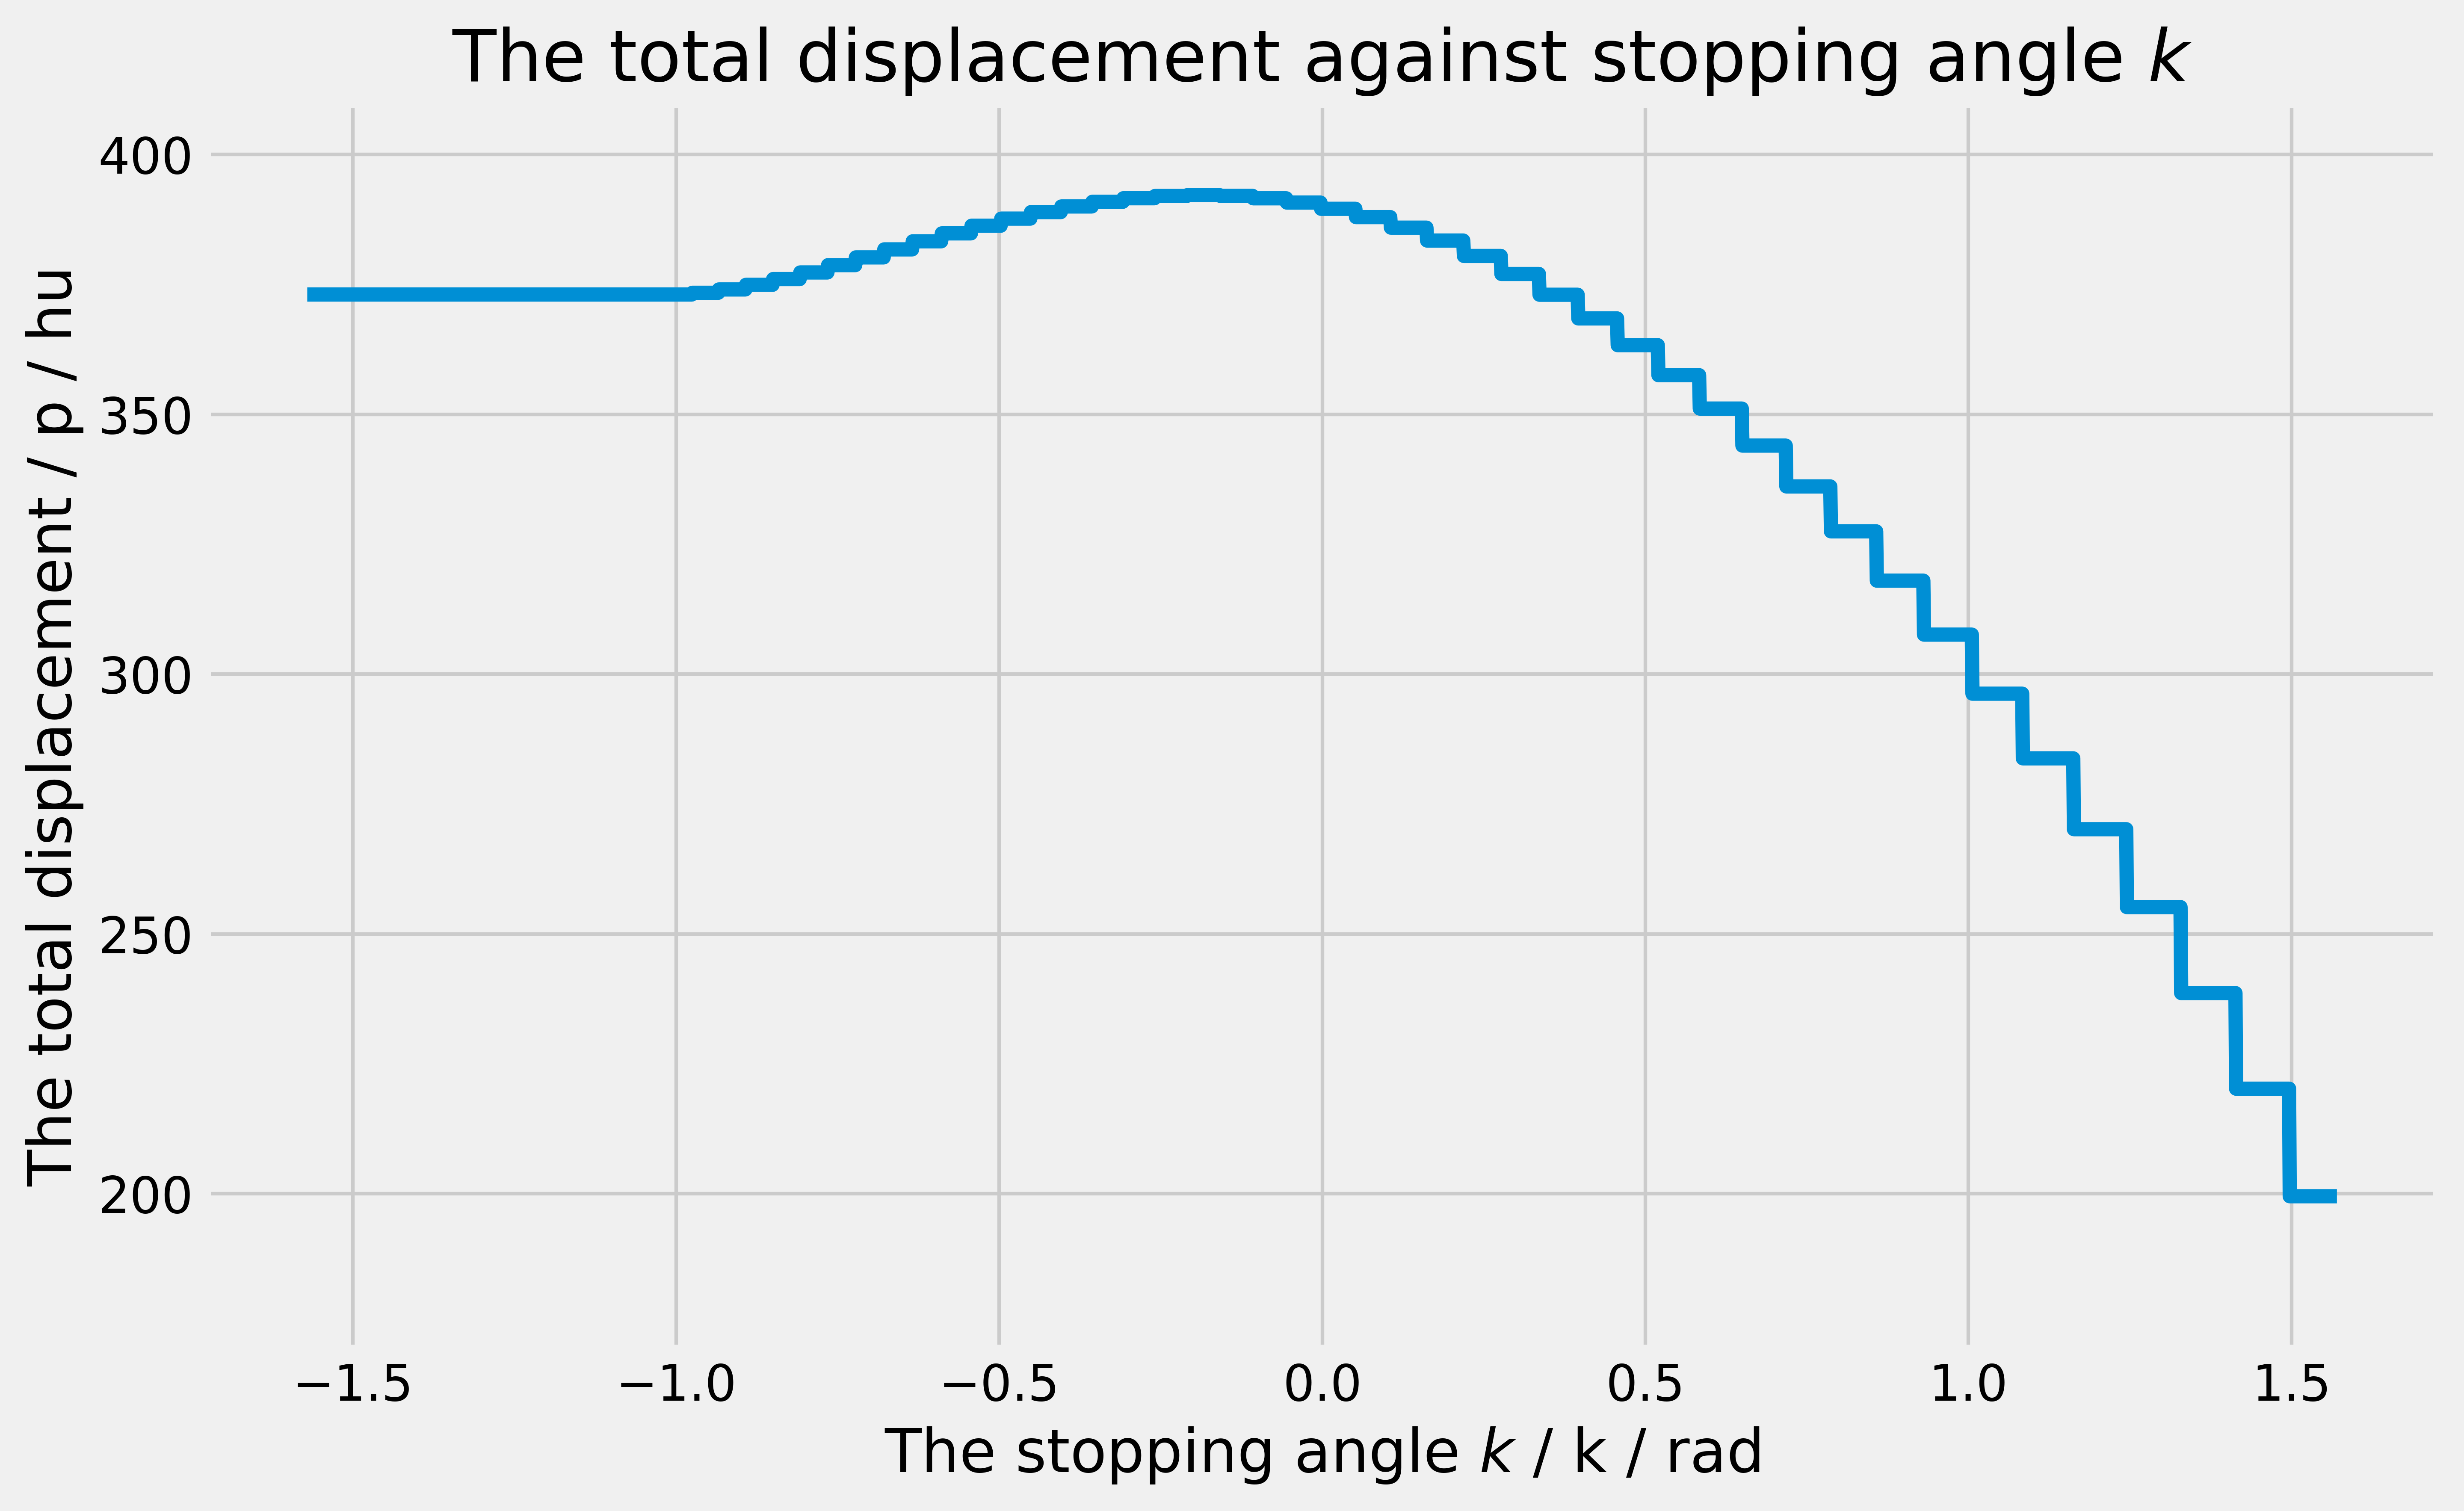
\includegraphics[width=0.8\textwidth]{assets/step_by_step_2k.png}
    \caption{}
    \label{fig:sbs2k}
\end{figure}

Yet this value of $k=-0.16$ is really stable judging by the low gradient around the local maxima in figure \ref{fig:sbs2k}. This allows for some error in the human player's stop turning angle, reducing the preciseness needed to perform this model and making it more accessibly without software assistance.

% the one where you accelerate below max value
% THIS IS CANCELLED DUE TO WORD LIMIT

%\subsubsection{Rotating initial velocity}
%To generalize the second discrete model, I wanted to utilize the rotational invariant of the problem to align the final displacement onto the x-axis.
%
%Because the model placed the player's final position at quite an angle against the initial velocity, it means that if we wish cross a gap, the intuitive assumption of initial velocity perpendicular to the ledge is incorrect for the player has turned. The first step of generalization would be finding the optimal angle of initial velocity.
%
%
%\begin{figure}[H]
%    \centering
%    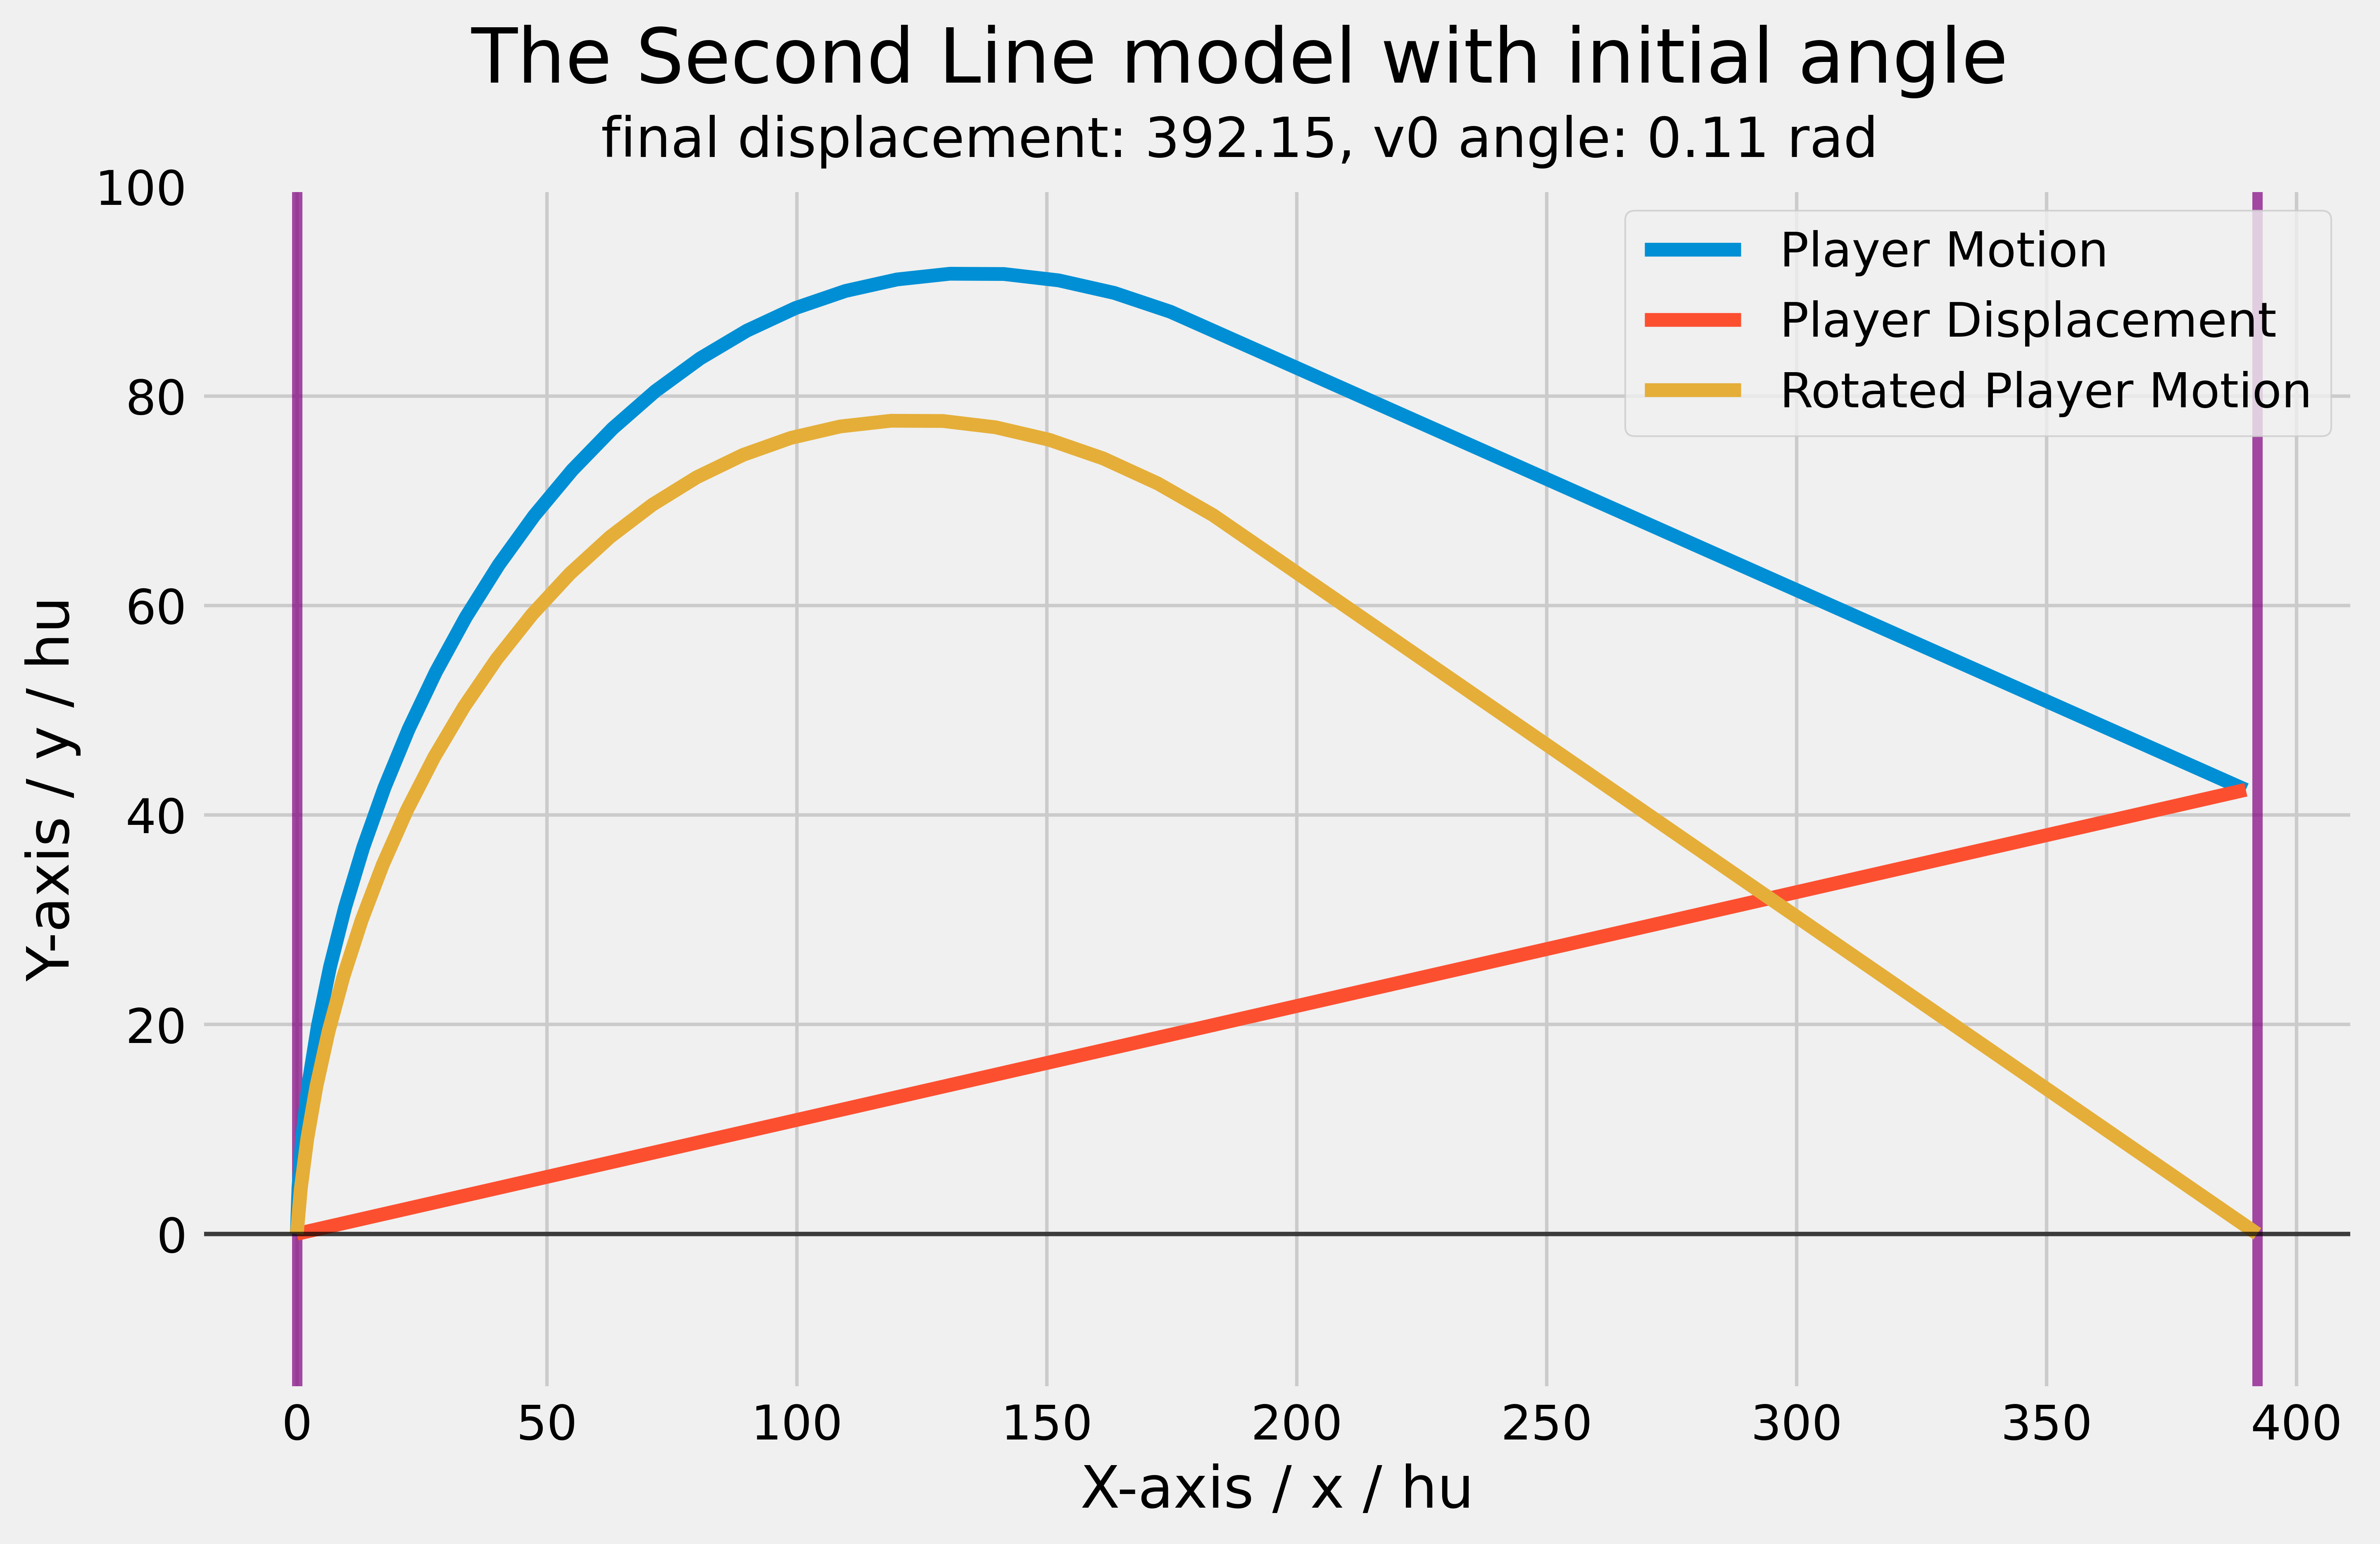
\includegraphics[width=0.8\textwidth]{assets/step_by_step_edge.png}
%    \caption{The rotation of the second discrete model}
%    \label{fig:sbsedge}
%\end{figure}
%
%
%Consider figure \ref{fig:sbsedge} with the x-axis gap as vertical purple lines. The blue curve represents the player motion with initial velocity in the y-axis
%\[
%    \tv(0) = \tang{0, 250},
%\]
%the red line is the final player's displacement. To ensure that the player's displacement is a line on the x-axis perpendicular to the gap, I can rotate the initial velocity (and thus entire player motion) by an angle $\phi$ so that the angle of the final displacement is zero. So
%\[
%    \phi = -\tan^{-1} \frac{42.4}{389.86} \approx -0.11,
%\]
%and the optimal player's initial velocity is
%\[
%    \tv_0 = R(\phi)\tpar{0}{250} = \begin{bmatrix}
%        \cos \phi & -\sin \phi \\
%        \sin \phi & \cos \phi
%    \end{bmatrix}\tpar{0}{250} \approx \tpar{27.03}{248.53}
%\]
%which is calculated by a 2d rotation matrix. The rotated player motion is the yellow curve in the figure above.

% 3866 words, very close
\subsection{Evaluation}
Overall, the second discrete model is a significant improvement over the first discrete model. It increased the total jump displacement from $\approx 373.0$ to $\approx 392.15$ due to the pausing of rotation at angle $\phi \approx -0.16$. I also found that the optimal initial velocity should be angled $\approx 0.11$ radians from the ledge if the player wishes to jump across the longest gap using the second discrete model:
\[
    \tan \frac{42.2}{389.86} \approx 0.11,
\]
because that is the angle of rotation needed to snap the jump endpoint to the x-axis.

\begin{figure}[H]
    \centering
    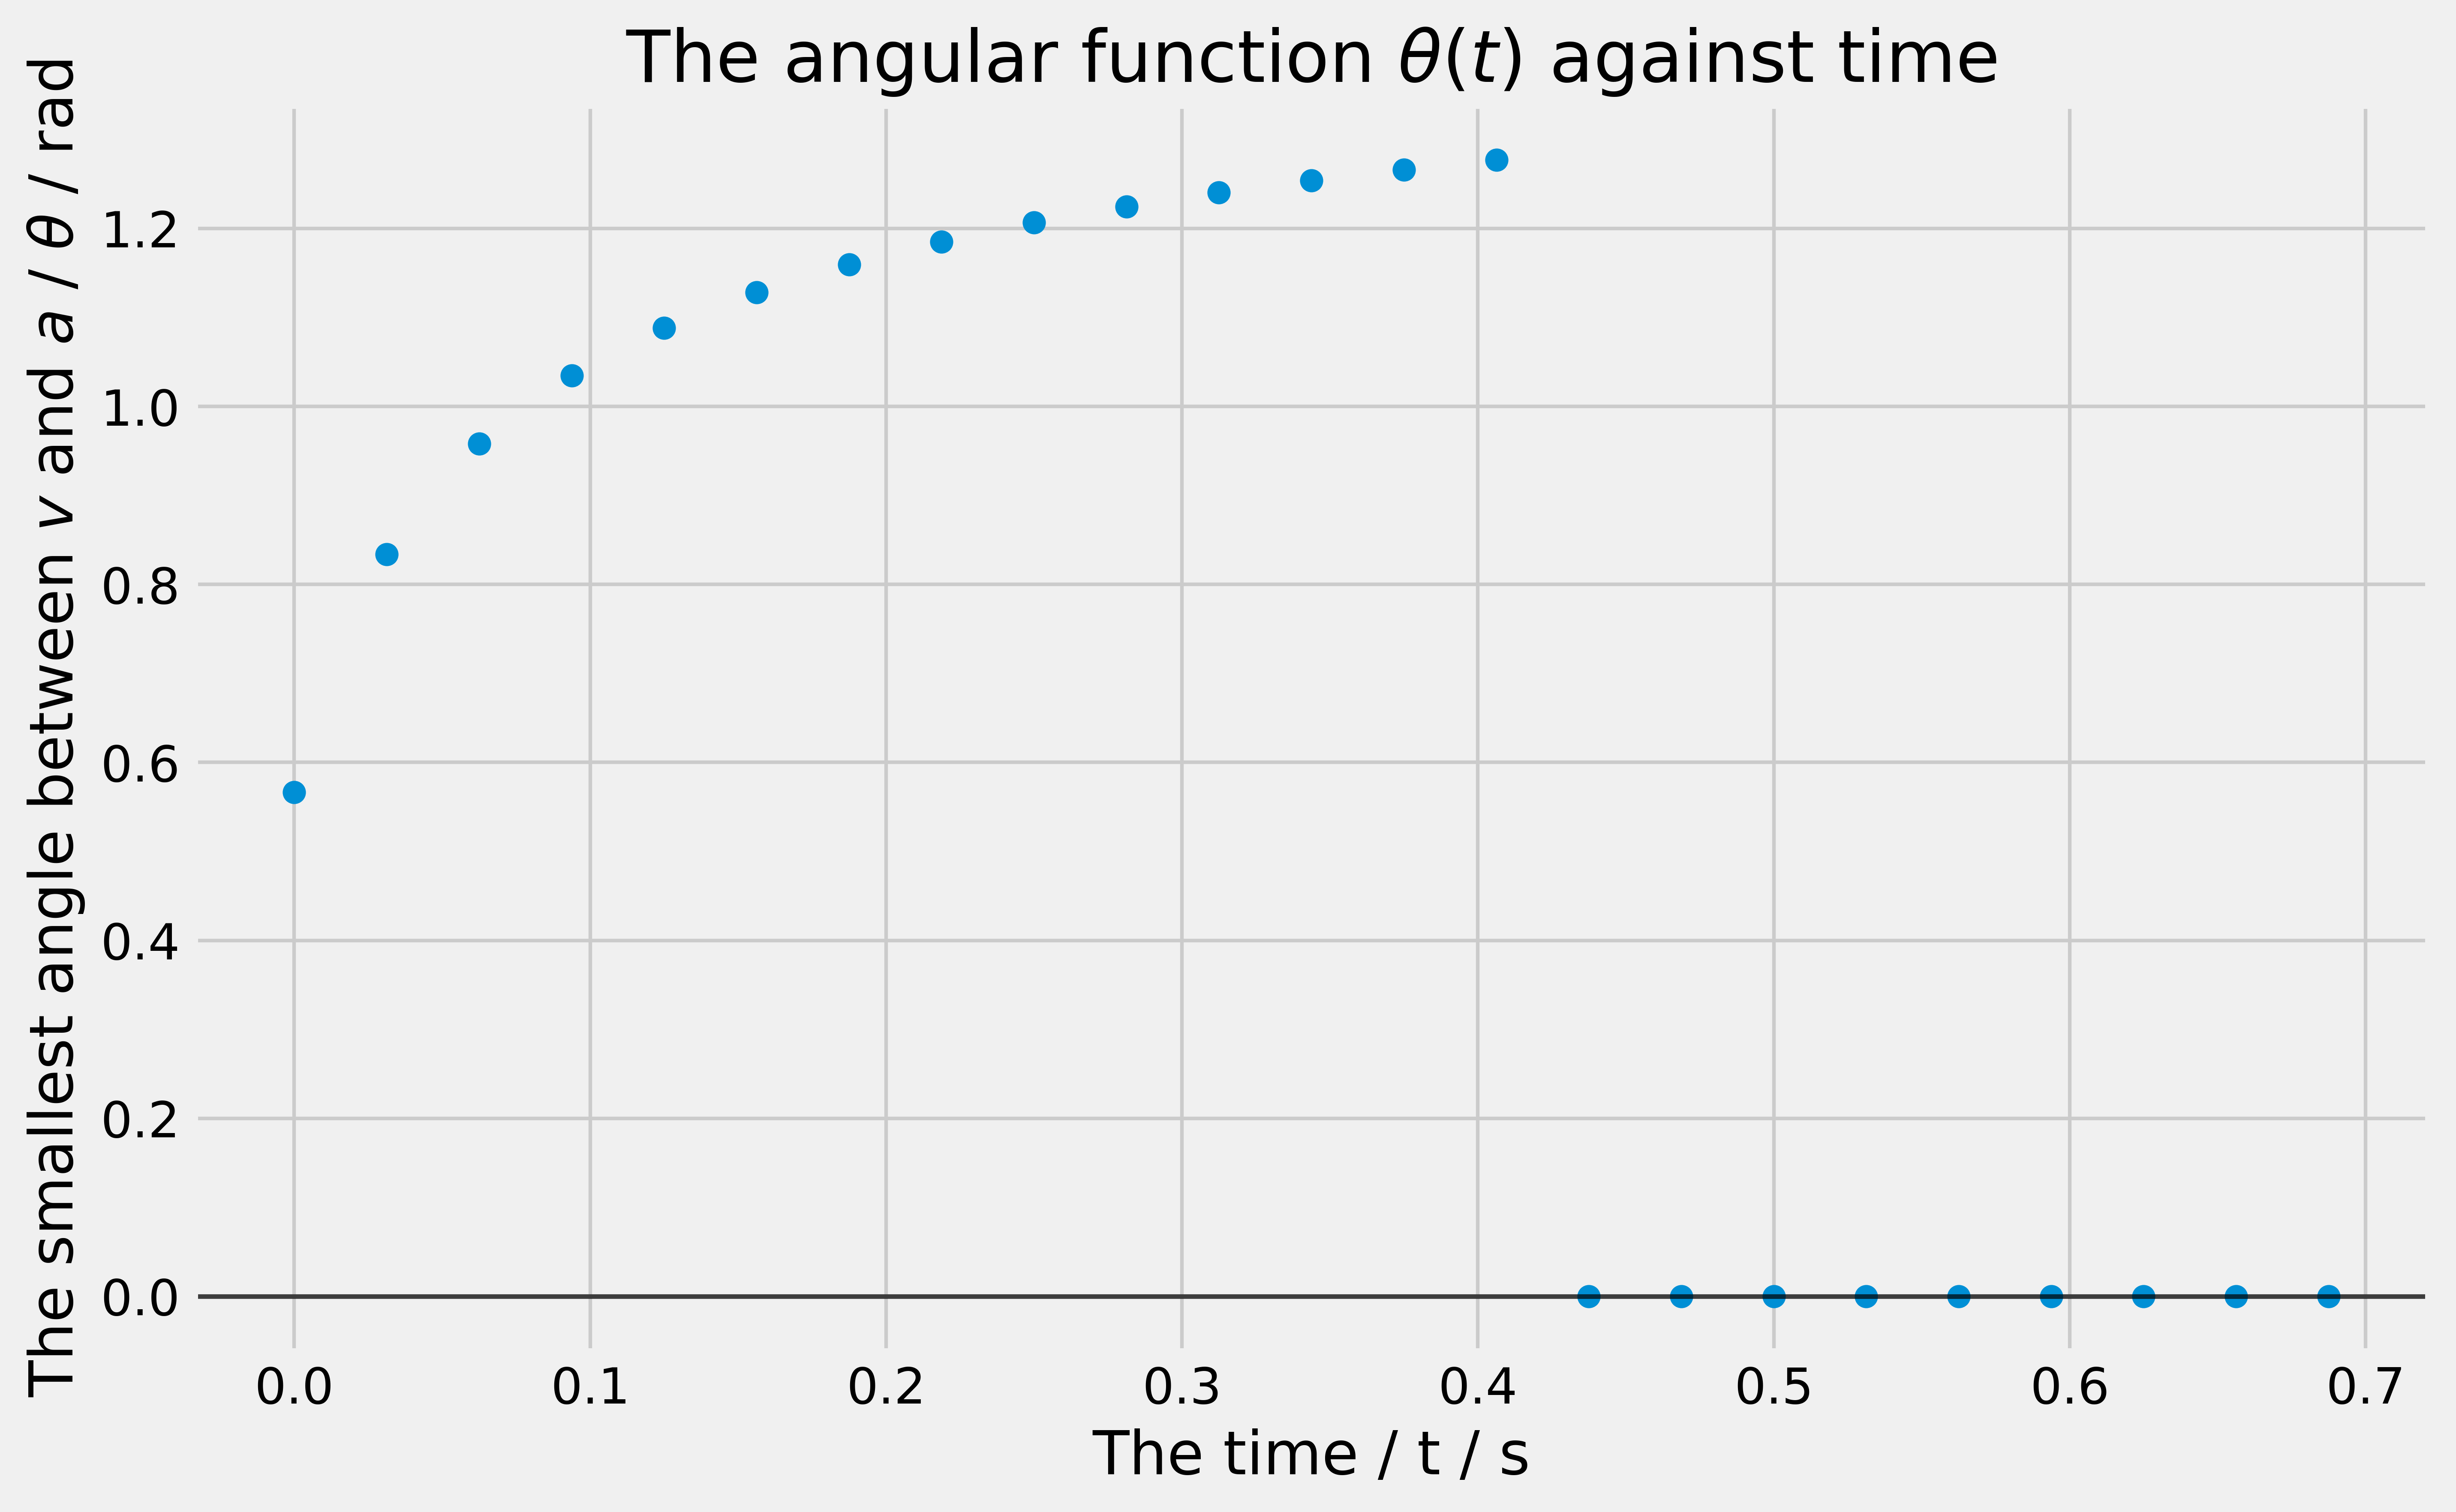
\includegraphics[width=0.8\linewidth]{assets/step_by_step_acc.png}
        \caption{The optimal discrete angular function $\theta(t)$}
        \label{fig:sbsa}
\end{figure}

%\begin{figure}[H]
%    \centering
%   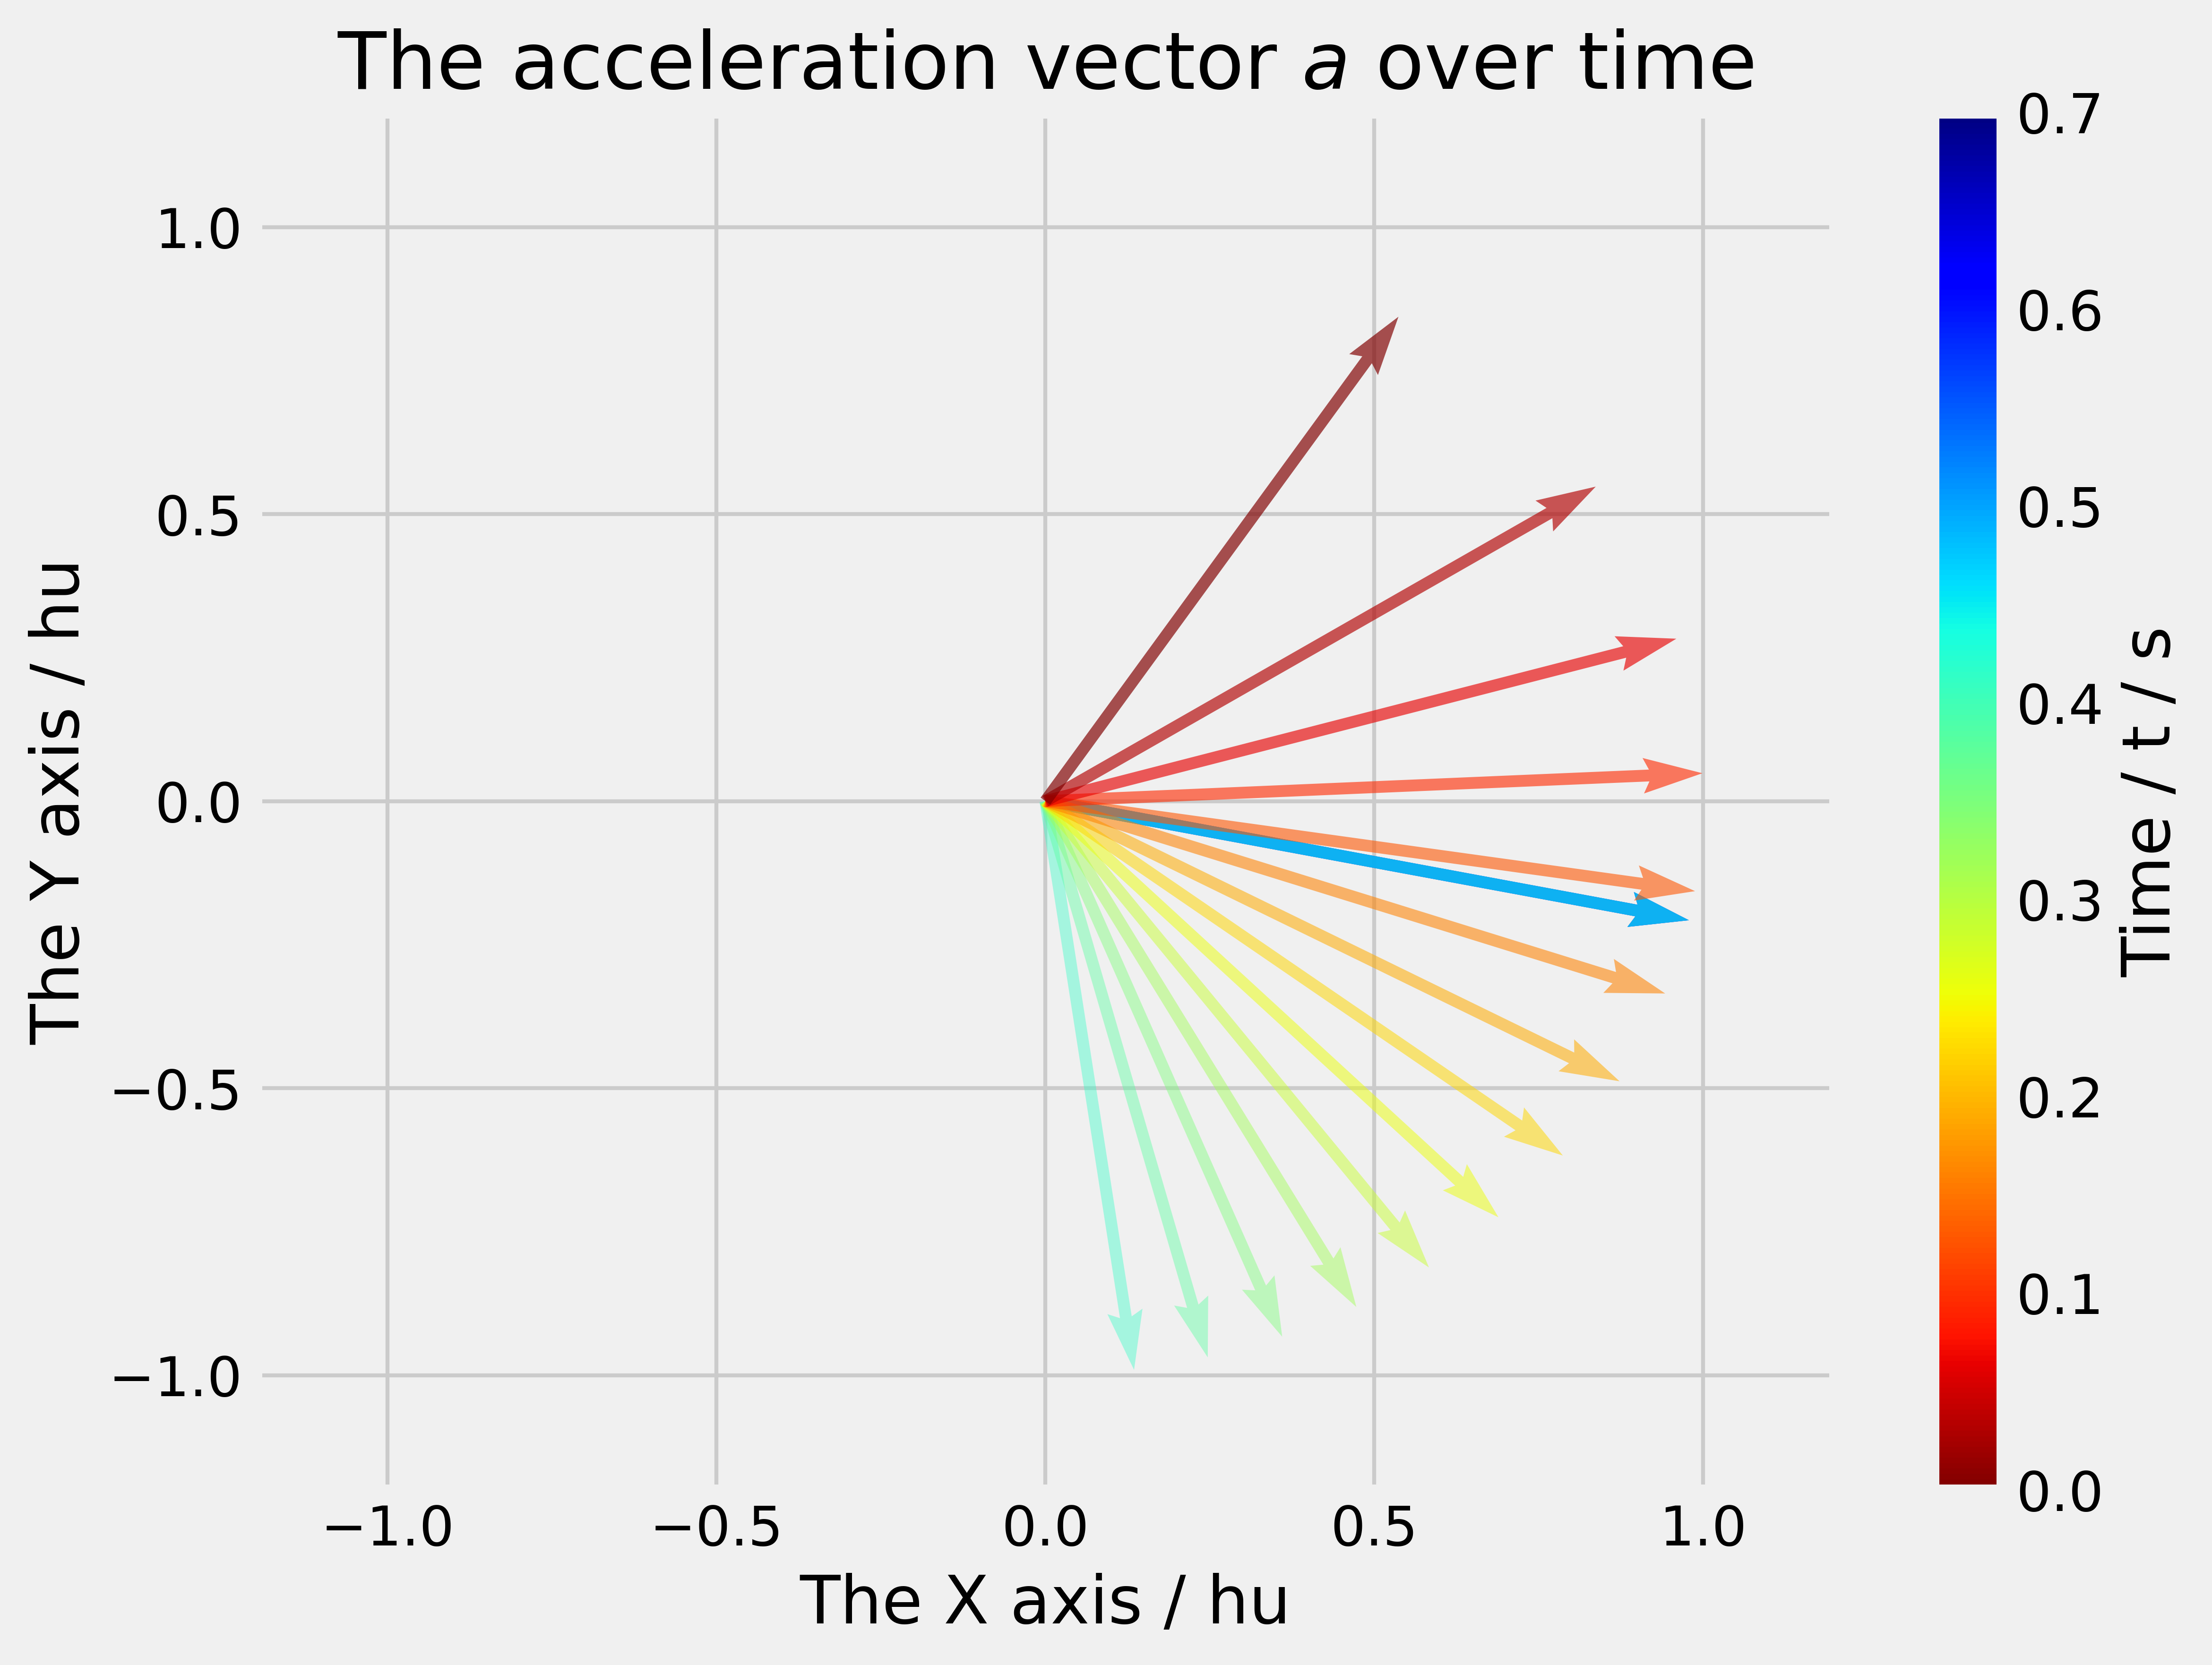
\includegraphics[width=0.7\linewidth]{assets/step_by_step_acc_v.png}
%        \caption{}
%        \label{fig:sbsav}
%\end{figure}

% conclusions
The discrete models overall are very complex and sophisticated for a player to achieve. The player must be able to judge their velocity, and accelerate at an increasing angle $\theta(t)$ over time against it as seen in figure \ref{fig:sbsa}. This is hard to achieve without external assistance from computers or software, but it grants a respective gain in jump displacement of around $200$ hammerunits against the simplest straight-line model.

The modification adds additional complexity in requiring the player to snap their acceleration as to stop any turning at a specific velocity angle, or at around $0.4$ seconds; but it comes with an extra gain of $392.15-373.0\approx19.15$ hammerunits of displacement against the non modified method, marking it the most optimal model I've came up with.
% conclude this method


